%%%%%%%%%%%%%%%%%%%%%%%%%%%%%%%%%%%%%%%%%%%%%%%%%%%%%%
% A Beamer template for University of Wollongong     %
% Based on THU beamer theme                          %
% Author: Qiuyu Lu                                   %
% Date: July 2024                                    %
% LPPL Licensed.                                     %
%%%%%%%%%%%%%%%%%%%%%%%%%%%%%%%%%%%%%%%%%%%%%%%%%%%%%%
% Customized for Sharif University of Technology     %
%%%%%%%%%%%%%%%%%%%%%%%%%%%%%%%%%%%%%%%%%%%%%%%%%%%%%%

\documentclass[serif, aspectratio=169]{beamer}
%\documentclass[serif]{beamer}  % for 4:3 ratio
\usepackage[T1]{fontenc} 
\usepackage{fourier} % see "http://faq.ktug.org/wiki/uploads/MathFonts.pdf" for other options
\usepackage{hyperref}
\usepackage[absolute,overlay]{textpos}
\usepackage{latexsym, amsmath, xcolor, multicol, booktabs, calligra}
\usepackage{graphicx, pstricks, listings, stackengine, caption, subcaption}
\usepackage{lipsum}

\author{Ali Sharifi-Zarchi}
\title{Machine Learning (CE 40477)}
\subtitle{Fall 2024}
\institute{
    CE Department \\
    Sharif University of Technology
}
%\date{\small \today}
% \usepackage{UoWstyle}
\usepackage{SUTstyle}

% defs
\def\cmd#1{\texttt{\color{red}\footnotesize $\backslash$#1}}
\def\env#1{\texttt{\color{blue}\footnotesize #1}}
\definecolor{deepblue}{rgb}{0,0,0.5}
\definecolor{deepred}{RGB}{153,0,0}
\definecolor{deepgreen}{rgb}{0,0.5,0}
\definecolor{halfgray}{gray}{0.55}

\lstset{
    basicstyle=\ttfamily\small,
    keywordstyle=\bfseries\color{deepblue},
    emphstyle=\ttfamily\color{deepred},    % Custom highlighting style
    stringstyle=\color{deepgreen},
    numbers=left,
    numberstyle=\small\color{halfgray},
    rulesepcolor=\color{red!20!green!20!blue!20},
    frame=shadowbox,
}


\begin{document}

\begin{frame}
    \titlepage
    \vspace*{-0.6cm}
    \begin{figure}[htpb]
        \begin{center}
            
\includegraphics[keepaspectratio, scale=0.25]{pic/sharif-main-logo}
        \end{center}
    \end{figure}
\end{frame}

\begin{frame}    
\tableofcontents[sectionstyle=show,
subsectionstyle=show/shaded/hide,
subsubsectionstyle=show/shaded/hide]
\end{frame}

\section{Why Deep Networks?}
\begin{frame}{Why Deep Networks? (Deep Expressivity)}
	\begin{textblock*}{5cm}(10.6cm, 2.5cm)
		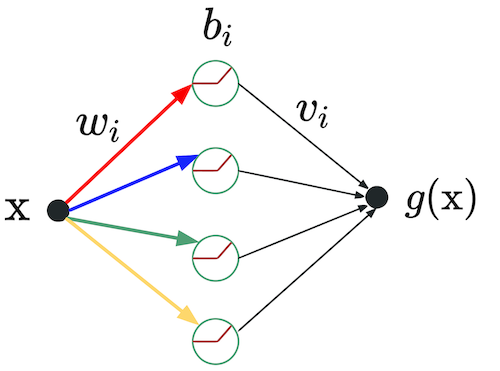
\includegraphics[keepaspectratio, scale=0.3]{pic/mlp}
	\end{textblock*}
	
	\begin{itemize}
		\item While the universal approximation theorem states that \newline a single-hidden-layer neural network can approximate \newline any function to a certain level of accuracy, it does not \newline specify how many hidden neurons are needed.
		\begin{itemize}
			\item It states there exists an integer $N$ and a set of \newline parameters $\{v_i,w_i,b_i\}_{i=1}^N$
			\item \textbf{Depth Separation Theorem:} For any integer $k>0$, \newline there exist neural networks with $\Theta(k^3)$ layers, $\Theta(1)$ \newline nodes per layer, and $\Theta(1)$ distinct parameters which \newline can't be approximated by networks with {O}$(k)$ layers \newline unless they are exponentially large (they must possess \newline $\Omega(2^k)$ nodes neurons).
		\end{itemize}
		
		\vspace{1cm}
		\scriptsize Telgarsky. Benefits of depth in neural networks. PMLR (2016).
	\end{itemize}
\end{frame}

\begin{frame}{Intuition}
	\begin{itemize}
		\item Let's consider ReLU networks. Let $m(x)$ be the \newline piecewise linear function as below: 
	\end{itemize}
	
	\begin{textblock*}{5cm}(2.8cm, 2.7cm)
		$$		
		\begin{aligned}
			m(x) = 
			\begin{cases}
				2x & 0 \le x \le 0.5\\
				2-2x & 0.5 \le x \le 1\\
				0 & o.w.\\
			\end{cases}
		\end{aligned}
		$$
	\end{textblock*}
	
	\vspace{2cm}
	\begin{itemize}
		\item This can be computed exactly by a two- or three- \newline layer network (depending on your notational \newline preferences), by the expression:
	\end{itemize}

	\begin{textblock*}{5cm}(3.6cm, 6.7cm)
		$\sigma (2 \sigma(x) - 4 \sigma(x - 0.5))$
	\end{textblock*}
	
	\vspace{0.5cm}
	\begin{itemize}
		\item Figure on the right shows it in terms of ReLU \newline activation functions
	\end{itemize}

	\begin{textblock*}{5cm}(10.3cm, 2.5cm)
		\begin{center}
			\begin{figure}
				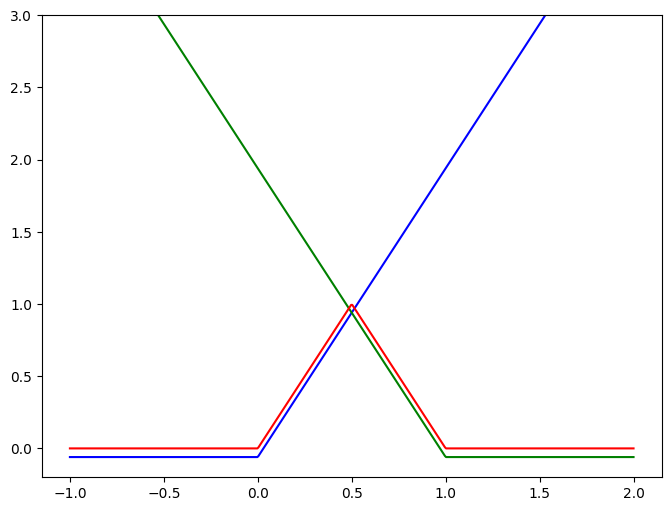
\includegraphics[keepaspectratio, scale=0.3]{pic/depth_sep_relu}
				\caption*{\tiny \hspace{1em} Function $m$ is slightly offset for visual clarity}
			\end{figure}
		\end{center}
	\end{textblock*}

\end{frame}

\begin{frame}{Intuition}
	\begin{textblock*}{5cm}(9.3cm,2cm) % {block width} (coords)
		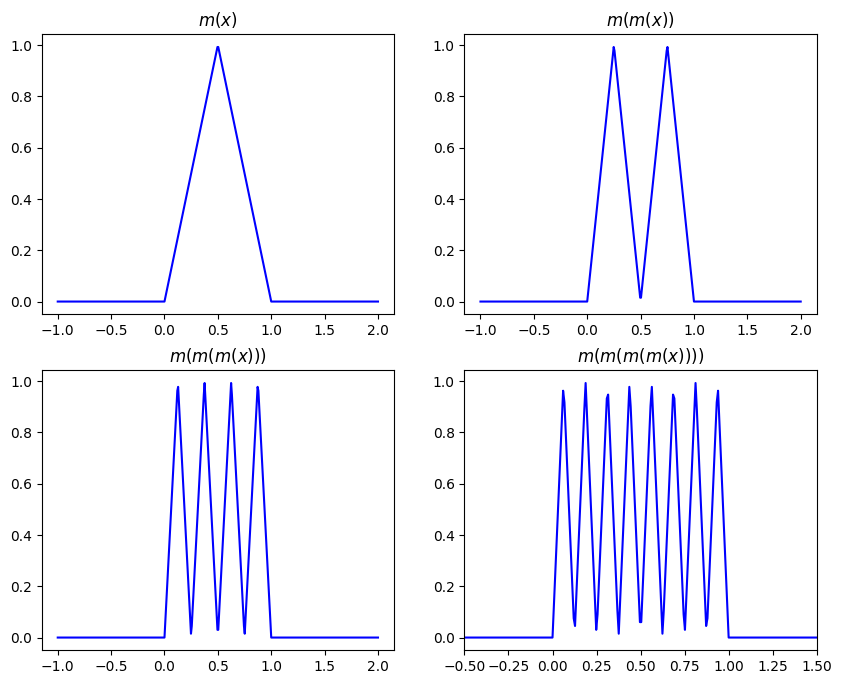
\includegraphics[keepaspectratio, scale=0.3]{pic/saw}
	\end{textblock*}
	\begin{itemize}
		\item What do iterates of $m(x)$ look like?
		\item So $m^{(n)}(x)$ would have $2^n$ “teeth”
		\item We can represent this function with $3n+1$ \newline nodes 
		\item A shallow network requires many nodes to \newline achieve this
		\item Depth increases the number of oscillations \newline multiplicatively whereas width can only do so \newline additively.
	\end{itemize}
	\hspace{1.3cm}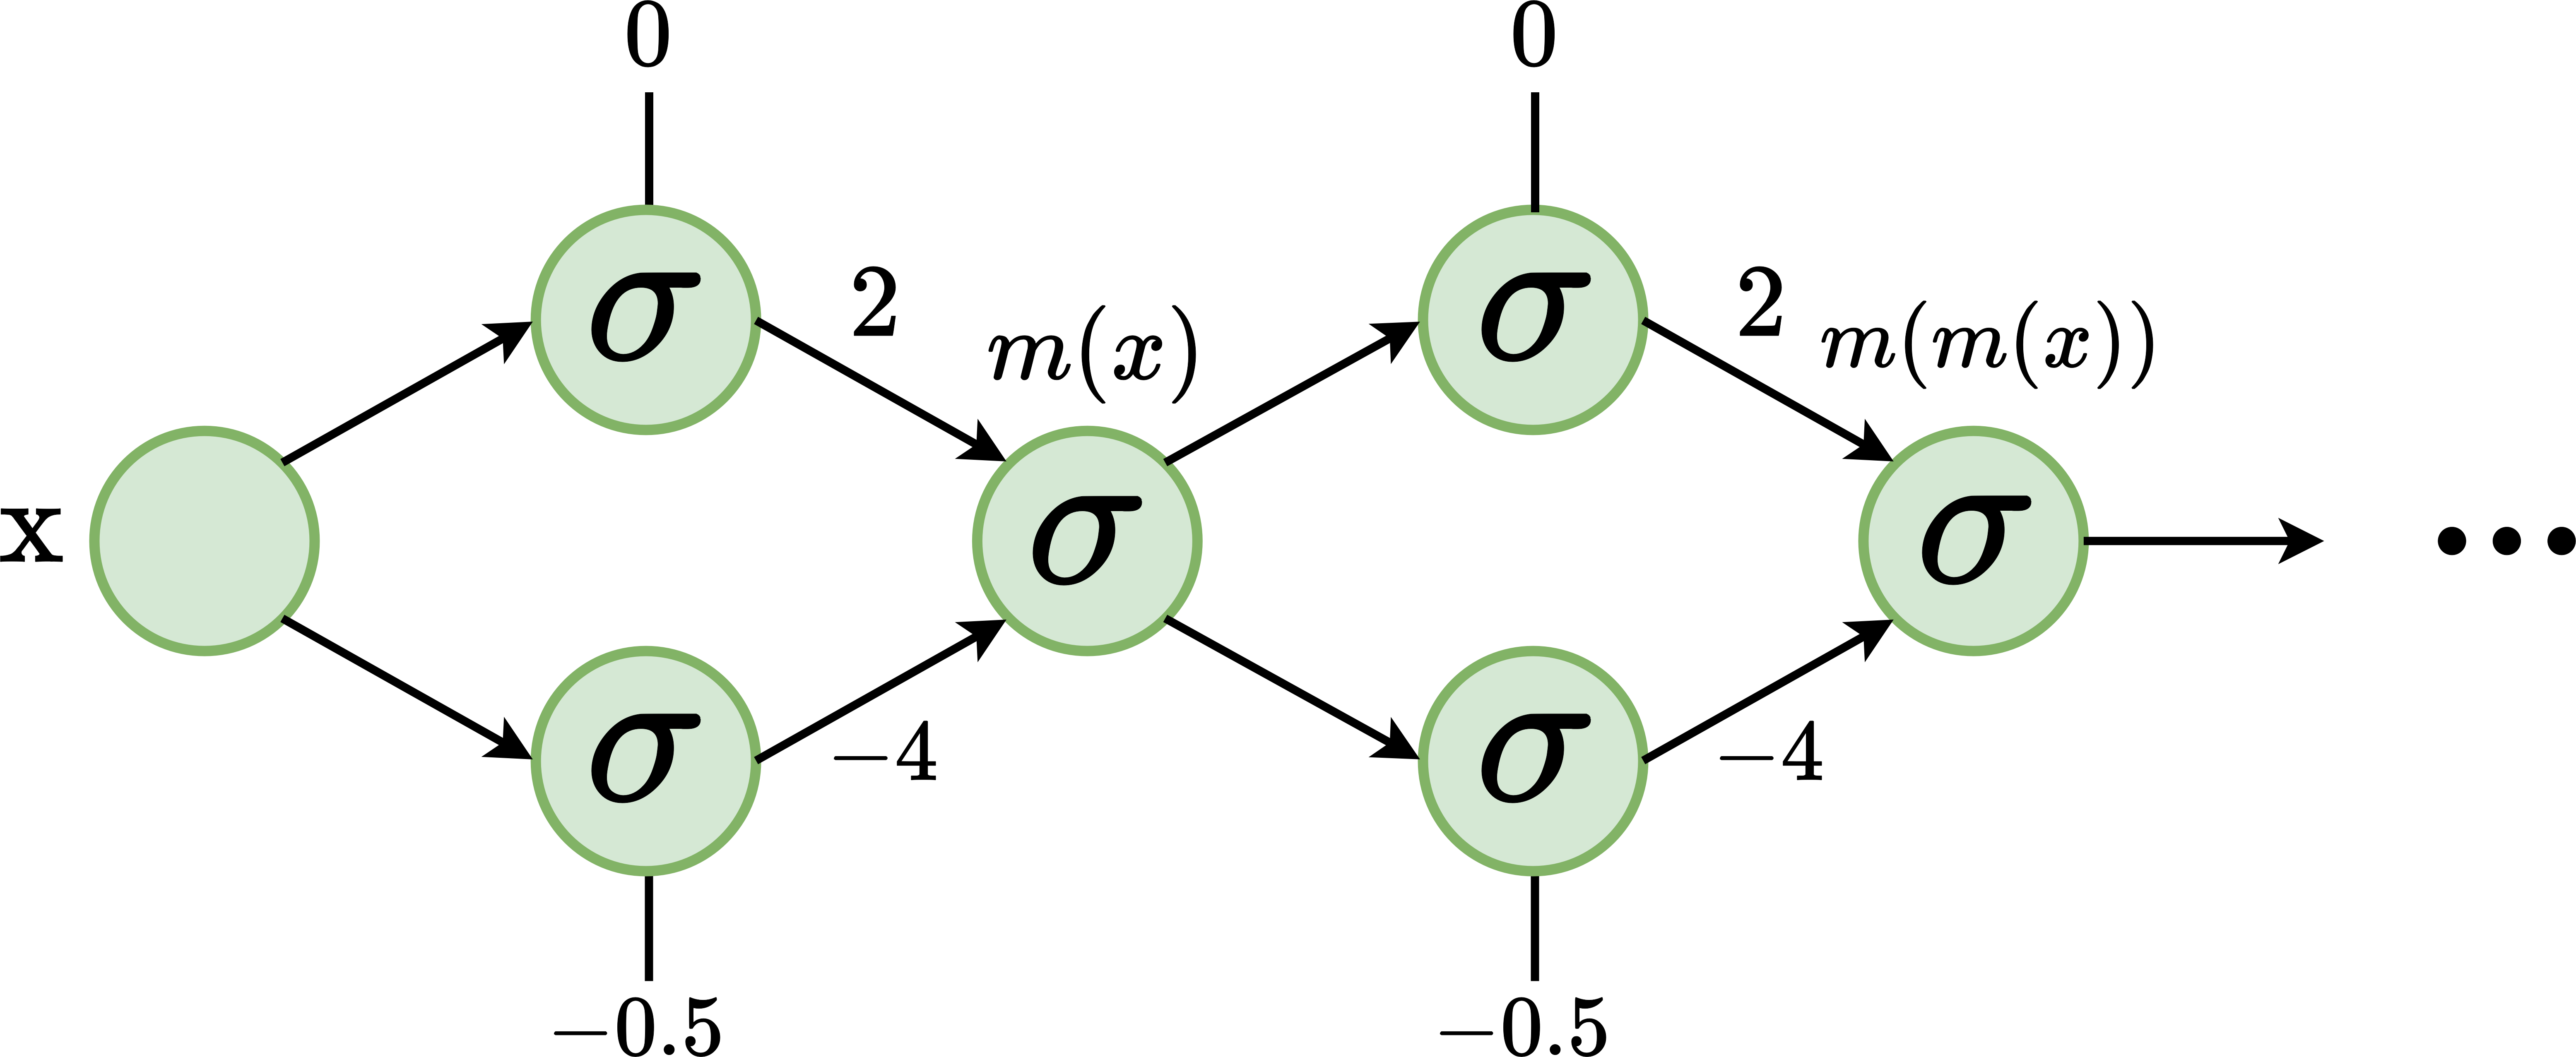
\includegraphics[keepaspectratio, width=6cm]{pic/2h}
\end{frame}

\section{AlexNet}
\begin{frame}{AlexNet [Krizhevsky, et al. NIPS (2012)]}
	\vspace{-1.3em}
	\textbf{Architecture:} \newline
	[$227 \times 227 \times 3$] INPUT \newline
	[$55 \times 55 \times 96$] \textcolor[rgb]{0.998, 0.007, 0.003}{CONV1 + ReLU}: 96 $11 \times 11$ filters at stride 4, pad 0 \newline
	[$27 \times 27 \times 96$] \textcolor[rgb]{0.001, 0.001, 0.998}{MAX POOL1}: MAX POOL1: $3 \times 3$ filters at stride 2 \newline
	[$27 \times 27 \times 96$] \textcolor[rgb]{0.219, 0.463, 0.114}{NORM1}: Normalization layer \newline
	[$27 \times 27 \times 256$] \textcolor[rgb]{0.998, 0.007, 0.003}{CONV2 + ReLU}: 256 $5 \times 5$ filters at stride 1, pad 2 \newline
	[$13 \times 13 \times 256$] \textcolor[rgb]{0.001, 0.001, 0.998}{MAX POOL2}: $3 \times 3$ filters at stride 2 \newline
	[$13 \times 13 \times 256$] \textcolor[rgb]{0.219, 0.463, 0.114}{NORM2}: Normalization layer \newline 
	[$13 \times 13 \times 384$] \textcolor[rgb]{0.998, 0.007, 0.003}{CONV3 + ReLU}: 384 $3 \times 3$ filters at stride 1, pad 1 \newline
	[$13 \times 13 \times 384$] \textcolor[rgb]{0.998, 0.007, 0.003}{CONV4 + ReLU}: 384 $3 \times 3$ filters at stride 1, pad 1 \newline
	[$13 \times 13 \times 256$] \textcolor[rgb]{0.998, 0.007, 0.003}{CONV5 + ReLU}: 256 $3 \times 3$ filters at stride 1, pad 1 \newline
	[$6 \times 6 \times 256]$ \textcolor[rgb]{0.001, 0.001, 0.998}{MAX POOL3}: $3 \times 3$ filters at stride 2 \newline
	[$4096$] \textcolor[rgb]{0.902, 0.570, 0.218}{Fully Connected 6 + ReLU} 4096 neurons \newline
	[$4096$] \textcolor[rgb]{0.902, 0.570, 0.218}{Fully Connected 7 + ReLU} 4096 neurons \newline
	[$1000$] \textcolor[rgb]{0.902, 0.570, 0.218}{Fully Connected 8} 1000 neurons (class scores) 

	\begin{textblock*}{5cm}(9.8cm, 6.5cm) % {block width} (coords)
		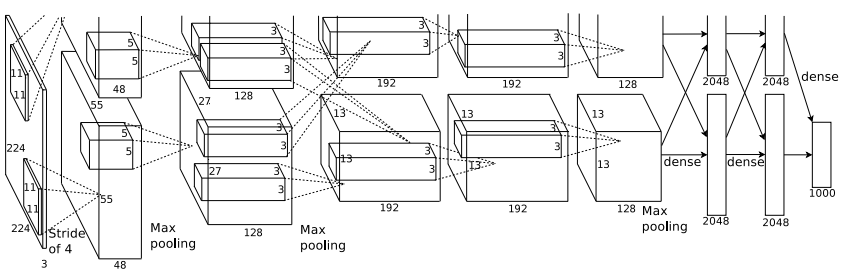
\includegraphics[keepaspectratio, width=5.9cm]{pic/alexnet}
	\end{textblock*}
\end{frame}

\begin{frame}{AlexNet At A Glance}
	\begin{figure}[htpb]
		\begin{center}
			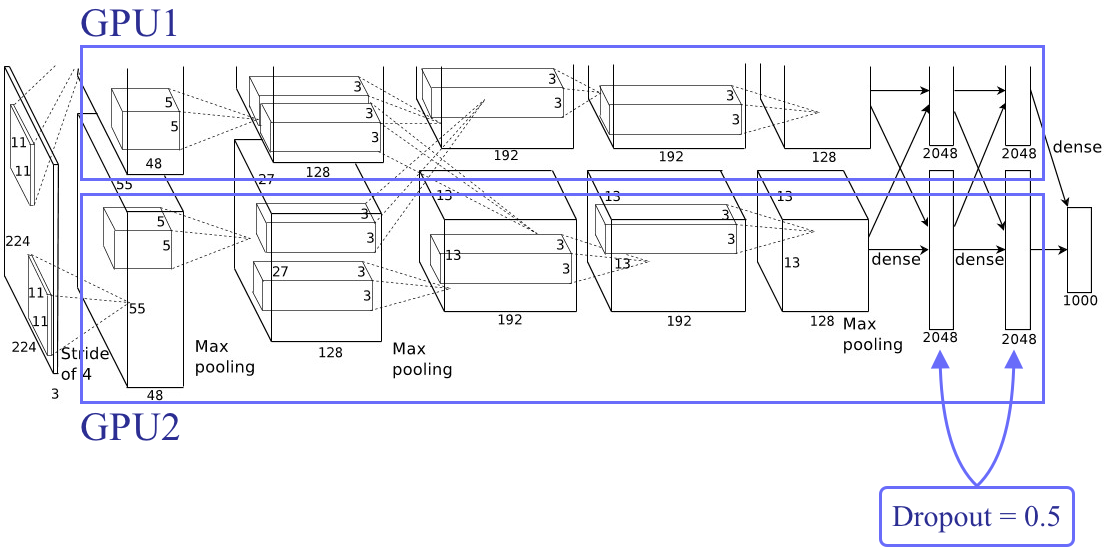
\includegraphics[keepaspectratio, scale=0.25]{pic/alexnet_annot}
		\end{center}
	\end{figure}
	\vspace{-0.2cm}
	\begin{itemize}
		\setlength{\itemsep}{-1.6pt}
		\item Training: 6 days on 2 NVIDIA GTX 580 GPUs (3 GB RAM)
		\item 8 layers / 60M parameters and 650K neurons
		\item Testing: Multi-crop
		\begin{itemize}
			\setlength{\itemsep}{-1.6pt}
			\item Classify different shifts of the image and vote over the lot!
			\item Test-time data augmentation
		\end{itemize}
	\end{itemize}
\end{frame}

\begin{frame}{Dropout}
	\begin{itemize}
		\item In each forward pass, randomly deactivate some neurons.
		\setbeamertemplate{itemize subitem}{$\rightarrow$}
		\begin{itemize}
			\item Probability of dropping is a hyperparameter $\Rightarrow$ 0.5 is common
			\item Gradients are computed only for the weights and biases between active nodes.
			\item For the remaining, the gradient is just 0.
		\end{itemize}
		\begin{figure}[htpb]
			\begin{center}
				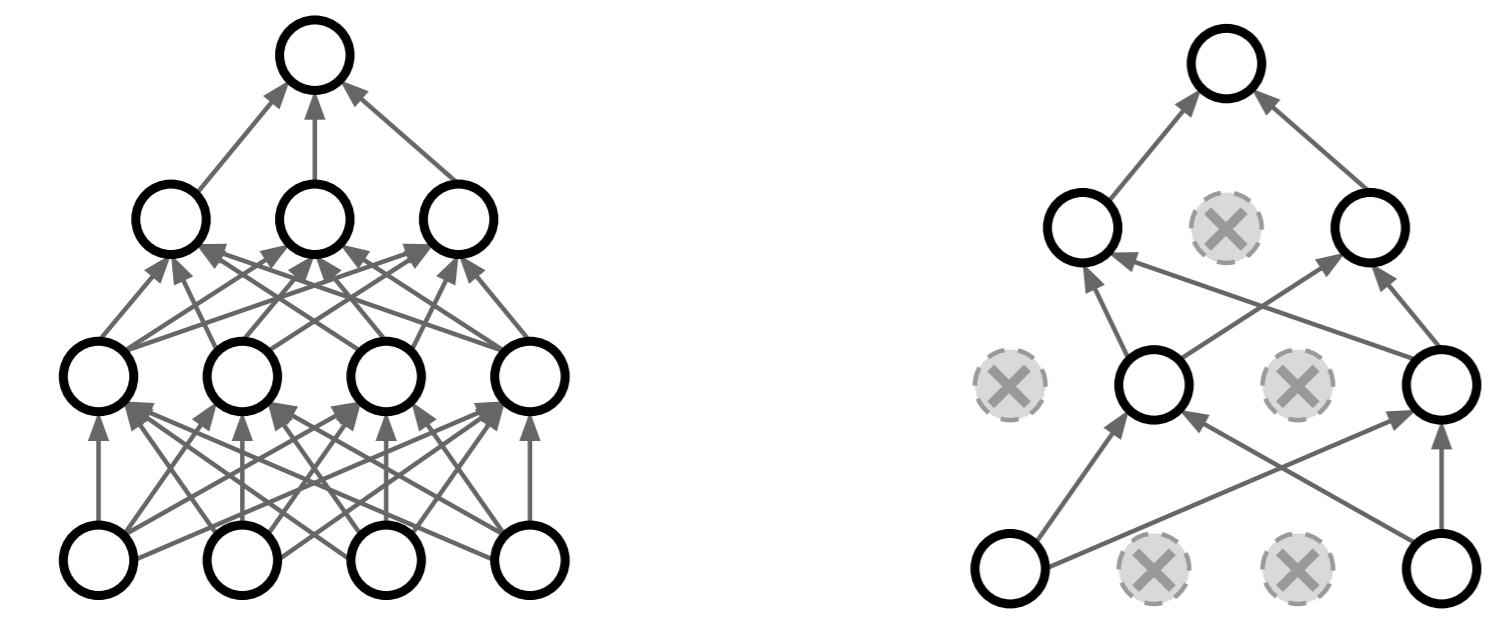
\includegraphics[keepaspectratio, scale=0.15]{pic/dropout}
				\caption*{\scriptsize Srivastava et al., JMLR 2014}
			\end{center}
		\end{figure}
		\vspace{-1em}
		\item Thus, a smaller network is trained for each sample.
		\setbeamertemplate{itemize subitem}{$\rightarrow$}
		\begin{itemize}
			\item Smaller network provides a regularization effect.
		\end{itemize}
	\end{itemize}
\end{frame}

\begin{frame}{ReLU}
	\textbf{ReLU}
	\begin{itemize}
		\item Does not saturate (in the positive region)
		\item Very computationally efficient
		\item Converges much faster than sigmoid/tanh \newline in practice (e.g. 6x)
		\item Actually more biologically plausible than sigmoid
		\item[{$\bullet$}] \textbf{Problems:}
		\setbeamertemplate{itemize subitem}{$\rightarrow$}
		\begin{itemize}
			\item Not zero-centered output
			\item An annoyance:
			\setbeamertemplate{itemize subsubitem}{$\star$}
			\begin{itemize}
				\item Hint: "what is the gradient when x < 0?"
			\end{itemize}
		\end{itemize}
	\end{itemize}
	\begin{textblock*}{5cm}(11cm,2.5cm) % {block width} (coords)
		\begin{figure}[htbp]
			\begin{center}
				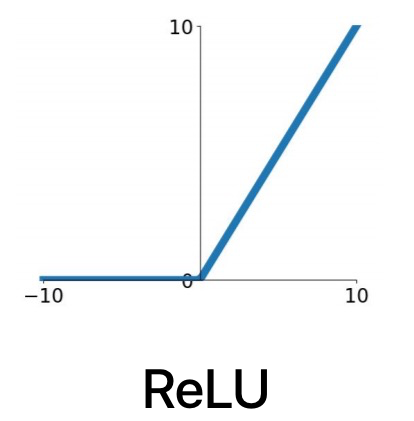
\includegraphics[keepaspectratio, scale=0.3]{pic/ReLU}
			\end{center}
		\end{figure}
	\end{textblock*}
\end{frame}

\begin{frame}{ReLU}
	\begin{itemize}
		\item ReLU trains faster than tanh.
	\end{itemize}
	\begin{figure}[htbp]
		\begin{center}
			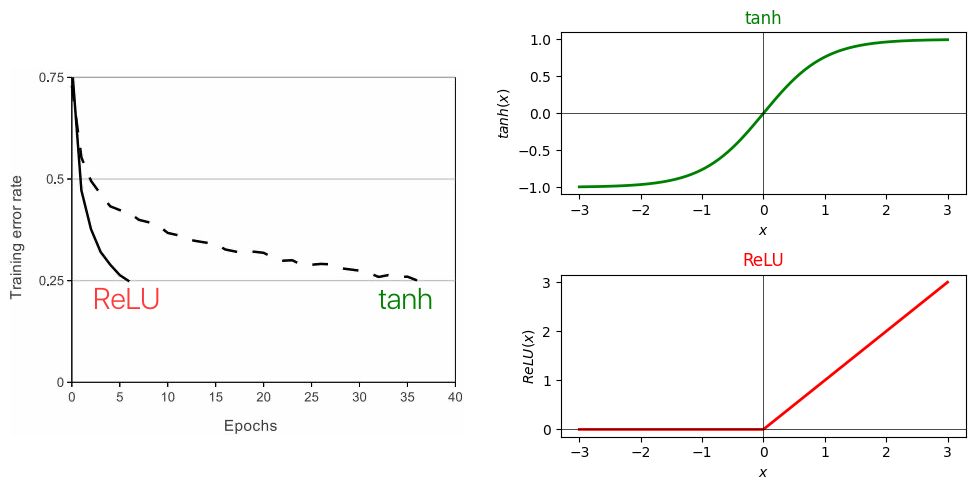
\includegraphics[keepaspectratio, scale=0.3]{pic/relu_faster}
			\caption*{\scriptsize Krizhevsky, et al., 2012}
		\end{center}
	\end{figure}
\end{frame}

\begin{frame}{Local Response Normalisation}
	\[
	b_{x, y}^i = \frac{a_{x, y}^i}{\left( k + \alpha \sum_{j=\max(0, i - \frac{n}{2})}^{\min(N - 1, i + \frac{n}{2})} \left( a_{x, y}^j \right)^2 \right)^\beta}
	\]
	\begin{itemize}
		\item Enhance the generalization of the model
		\item Encourages competition between adjacent features
		\vspace{1em}
		\begin{itemize}
			\item \( b_{x, y}^i \): Normalized activation at spatial location \((x, y)\) in the \(i\)-th channel.
			\item \( a_{x, y}^i \): Original activation at the same location and channel.
			\item \( N \): Total number of channels.
			\item \( n \): Size of the local neighborhood (number of adjacent channels to consider for normalization).
			\item \( k, \alpha, \beta \): Hyperparameters controlling the normalization.
		\end{itemize}
	\end{itemize}
\end{frame}

\begin{frame}{Learning Magic In Alexnet}
	\begin{itemize}
		\item First use of ReLU
		\setbeamertemplate{itemize subitem}{$\rightarrow$}
		\begin{itemize}
			\item Made a large difference in convergence
		\end{itemize}
		\item Dropout probability 0.5 (in FC layers only)
		\item Augmentations: translation, horizontal flip, altering the intensities of the RGB channels
		\item SGD with momentum of 0.9 and a mini-batch size of 128
		\item L2 weight decay 5e-4 ($l=l_{data} + \lambda||w||^2$)
		\item Learning rate: 0.01, decreased by 10 every time validation accuracy plateaus
		\item Evaluation metric: Validation accuracy
		\item \textbf{Final top-5 error: 18.2\% with a single net, 15.4\% using an ensemble of 7 networks}
		\setbeamertemplate{itemize subitem}{$\rightarrow$}
		\begin{itemize}
			\item \textbf{Lowest prior error using conventional classifiers: > 25 \%}
		\end{itemize}
	\end{itemize}
\end{frame}

\section{ResNet}

\begin{frame}{Revolution Of Depth}
	\begin{figure}[htpb]
		\begin{center}
			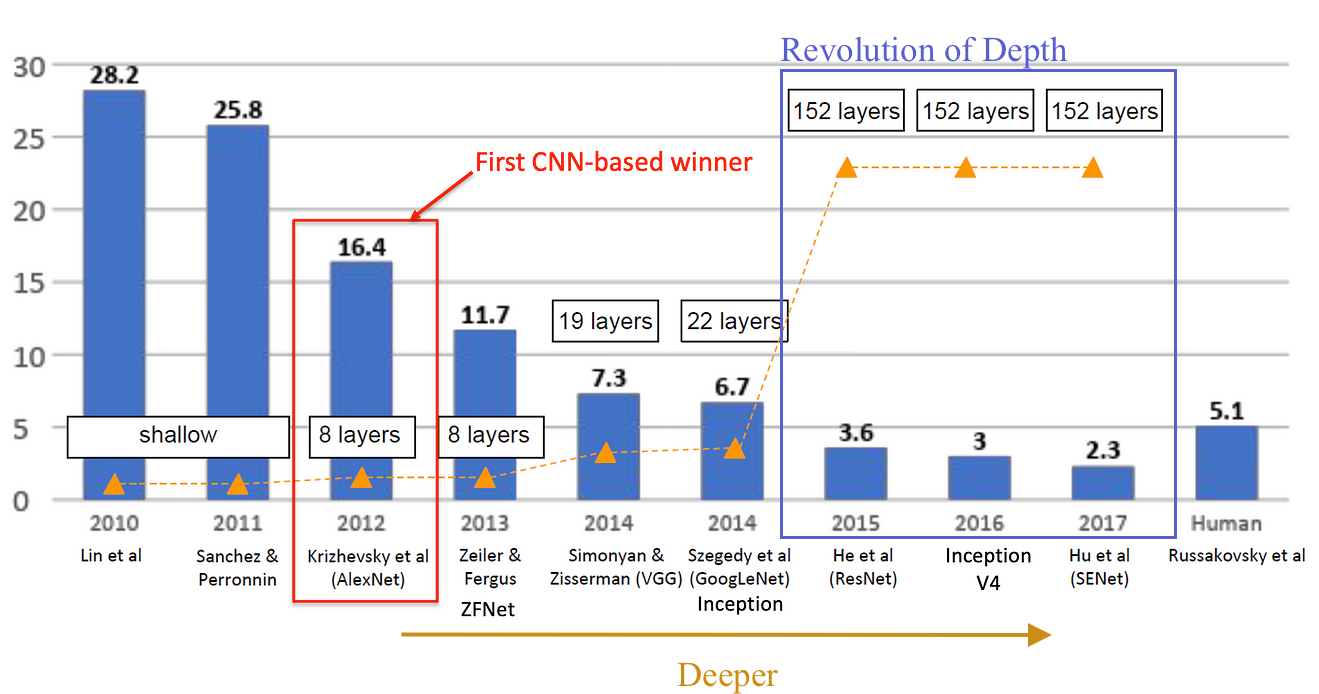
\includegraphics[keepaspectratio, scale=0.25]{pic/resnet-chart}
		\end{center}
	\end{figure}
\end{frame}

\begin{frame}{Challenge Of Making CNNs Deeper}
	\begin{itemize}
		\item What happens when we continue stacking deeper layers on a convolutional neural network?
		\item \textbf{Question}: What is strange about these training and test curves?
	\end{itemize}
	\begin{figure}[htpb]
		\begin{center}
			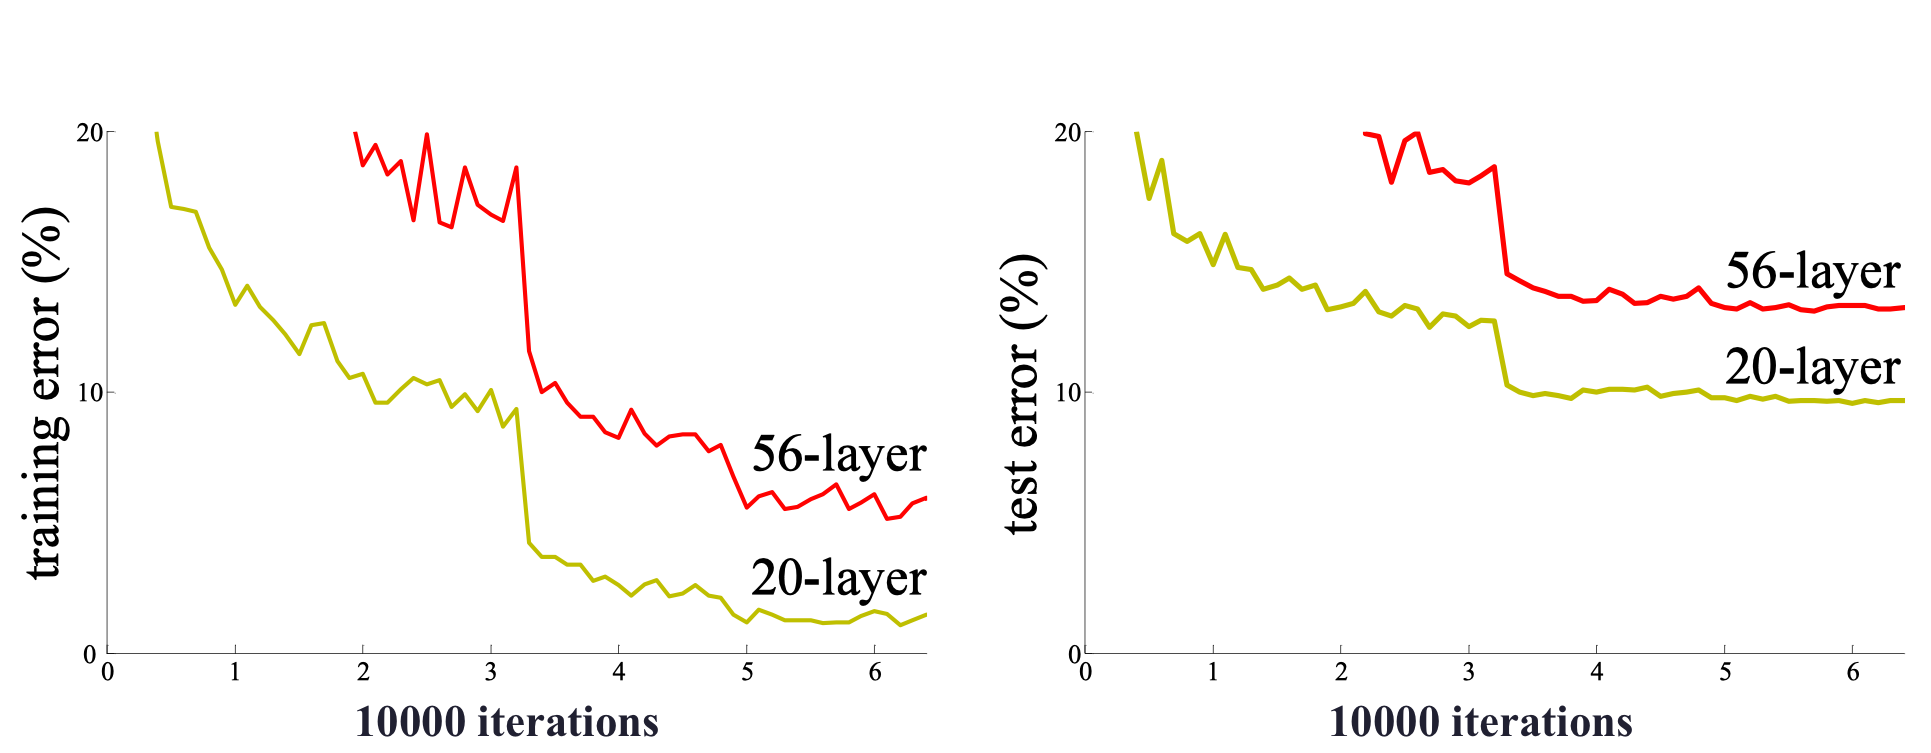
\includegraphics[keepaspectratio, scale=0.17]{pic/plain}
			\captionsetup{justification=centering}
			\caption*{\scriptsize{Training error (left) and test error (right) on CIFAR-10 with 20-layer and 56-layer “plain” networks}}
		\end{center}
	\end{figure}
\end{frame}

\begin{frame}{Challenge Of Making CNNs Deeper}
	\begin{itemize}
		\item \textbf{Fact:} Deeper models have minotore representation power (more parameters) than shallower models.
		\item But \textbf{56-layer model performs worse} on both training and test error and it's not caused by overfitting!
		\item \textbf{Hypothesis:} The issue is related to optimization, deeper models are harder to optimize.	
	\end{itemize}
	\vspace{-0.5cm}
	\centering
	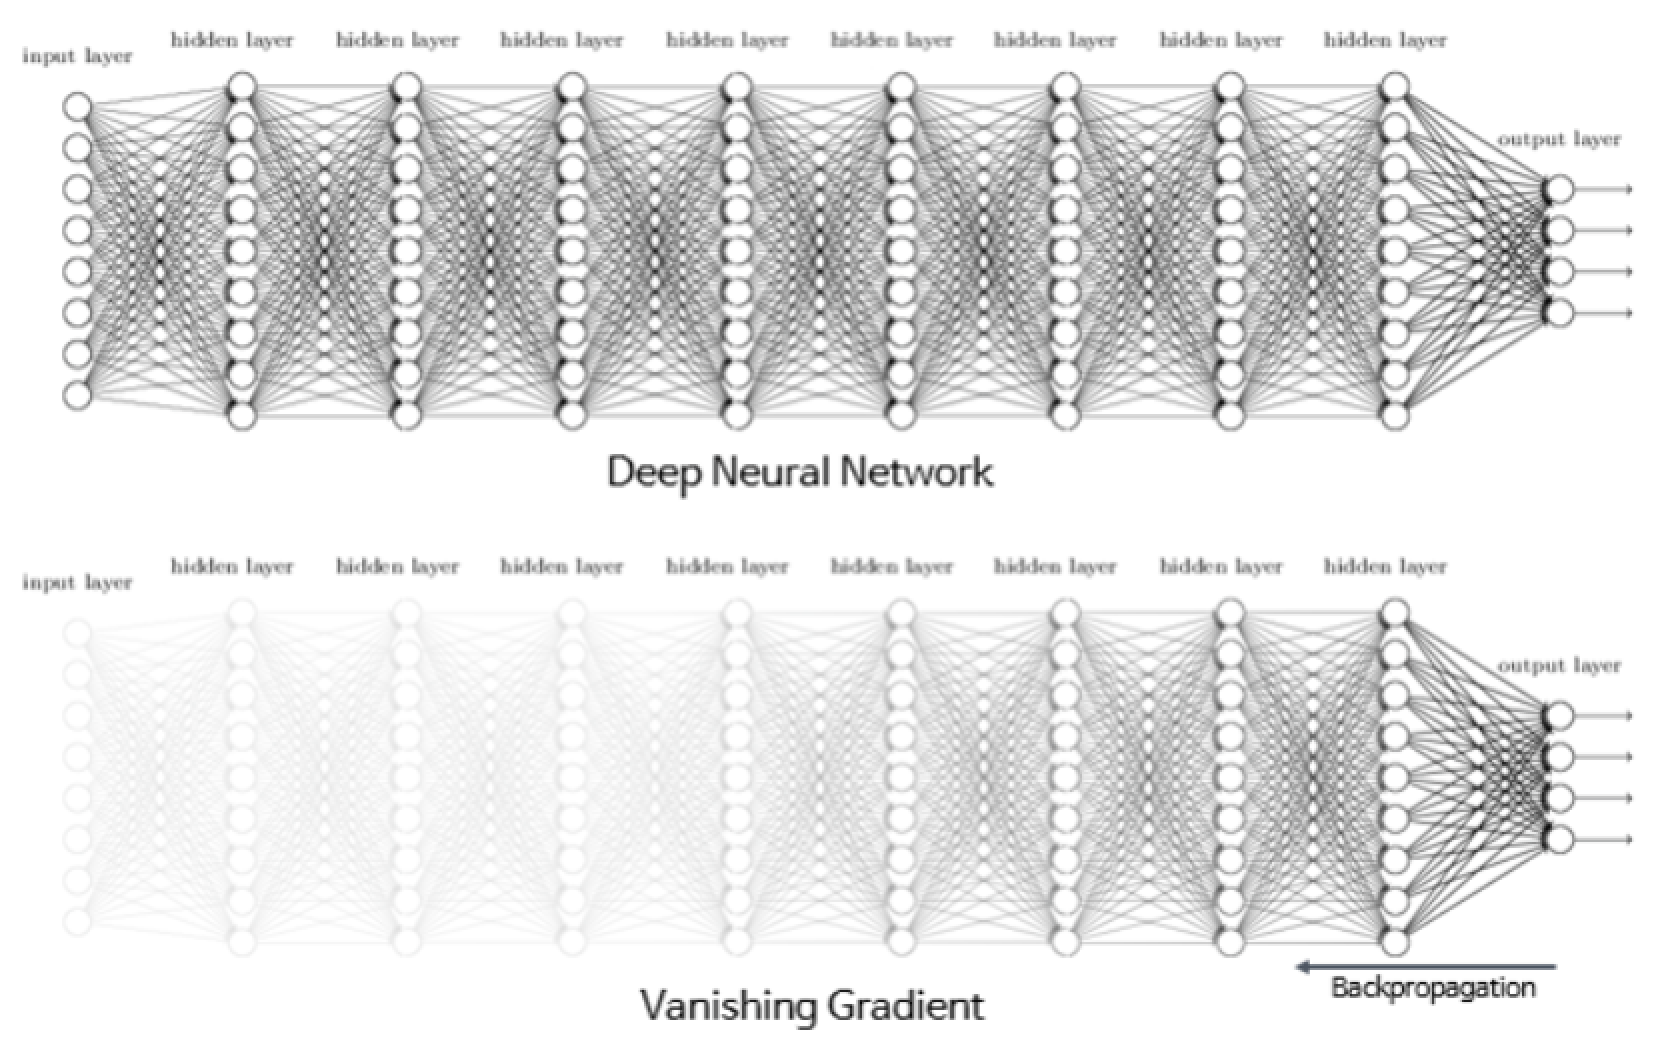
\includegraphics[keepaspectratio, scale=0.23]{pic/vanish}
\end{frame}

\begin{frame}{Residual Block}
	
	\begin{itemize}
		\item \textbf{Solution:} Use network layers to fit a residual mapping rather than directly fitting the desired underlying mapping.
		\item Identity mapping: $H(\mathbf{x}) = \mathbf{x} \ \text{if} \  F(\mathbf{x}) = 0$
	\end{itemize}
	
	\begin{figure}[htpb]
		\begin{center}
			\hspace{2cm} 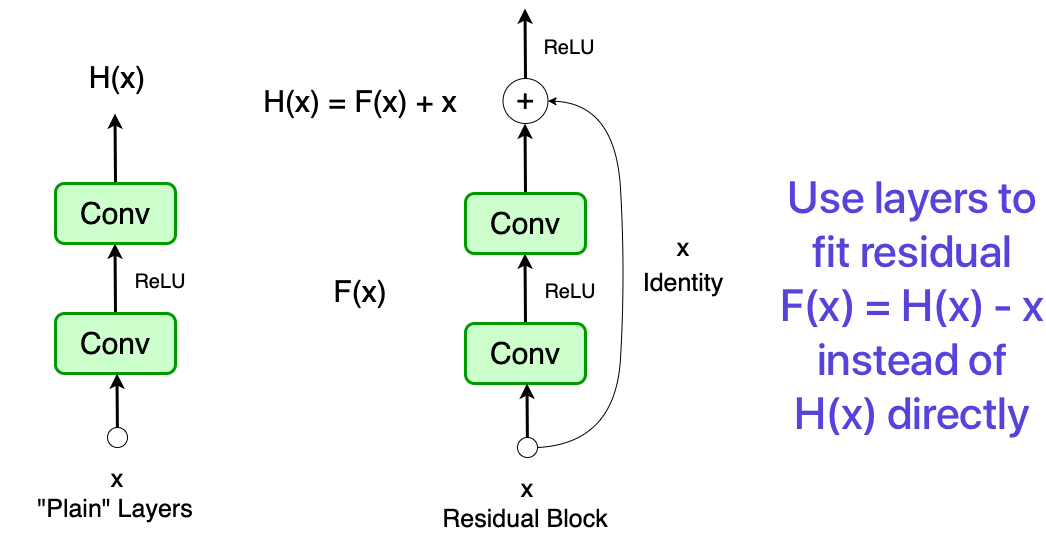
\includegraphics[keepaspectratio, scale=0.24]{pic/resBlock2}
		\end{center}
	\end{figure}

\end{frame}

\begin{frame}{Backpropagation In Residual Block}
	\begin{itemize}
		\item How exactly does the skip connection \newline prevent gradient vanishing?
		\item \textbf{During backpropagation, there are two pathways.}
	\end{itemize}
	
	\begin{textblock*}{5cm}(10.5cm,2cm) % {block width} (coords)
		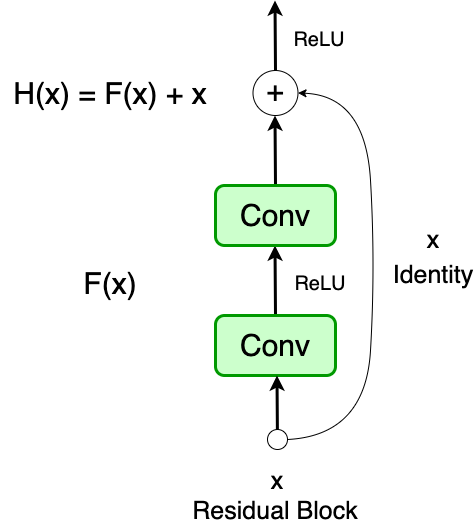
\includegraphics[keepaspectratio, scale=0.3]{pic/resBlock3}
	\end{textblock*}

    \begin{textblock*}{10cm}(1.3cm, 4cm) 
		$$			
		\begin{aligned}
			H(x) & = F(x) + x \\
			\frac{\partial L}{\partial x} & = \frac{\partial L}{\partial H} \times \frac{\partial H}{\partial x} = \frac{\partial L}{\partial H} \times \left( \frac{\partial F}{\partial x} + 1 \right) = \frac{\partial L}{\partial H} \times \frac{\partial F}{\partial x} + \frac{\partial L}{\partial H} \\
		\end{aligned}
		$$
	\end{textblock*}
	
	\vspace{2.2cm}
	\begin{itemize}
		\item If the gradient of Path 1 vanishes to 0, the gradient of \newline Path 2 still remains non-zero (because this gradient \newline  does not encounter any weight layer)
	\end{itemize}
\end{frame}

\begin{frame}{ResNet [He, et al., (2015)]}
	\begin{textblock*}{5cm}(8.8cm,1.7cm) % {block width} (coords)
		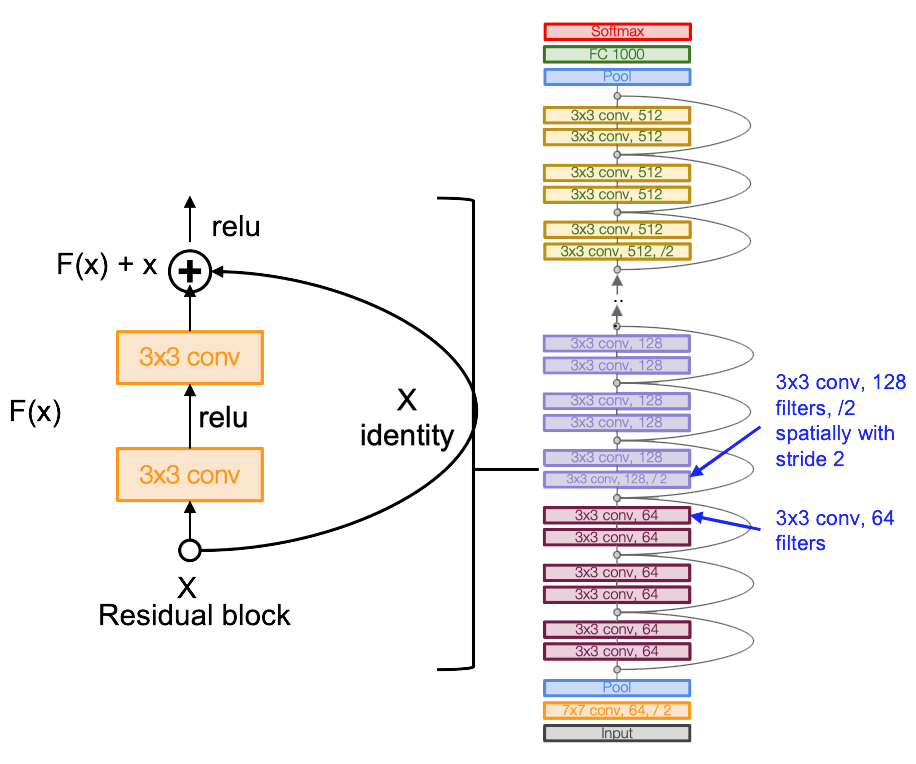
\includegraphics[keepaspectratio, scale=0.22]{pic/res_arch}
	\end{textblock*}
	\textbf{Architecture:}
	\begin{itemize}
		\item Stack of residual blocks
		\item Doubling the filter count while halving \newline spatial dimensions (via stride-2) at regular \newline intervals in the network Reduce the \newline activation volume by half.
		

		\item One FC layer at the end to output classes
		\item Total depths of 18, 34, 50, 101, or 152 \newline layers for ImageNet
	\end{itemize}
\end{frame}

\begin{frame}{Deeper Residual Module (Bottleneck)}
	\begin{itemize}
		\item For deeper networks (ResNet- 50+), use \newline ``bottleneck'' layer instead, to improve \newline efficiency.
		\item Bottleneck uses 1x1 convolution to:
		 \begin{itemize}
		 	\item Reduce number of paramters
		 	\item Enable interaction between channels, \newline creating new feature representations at \newline each spatial location
		 	\item Allow more layers to be added without \newline a significant increase in computational \newline cost or overfitting risk.
		 \end{itemize}
	\end{itemize}

	\begin{textblock*}{5cm}(8.7cm,1.9cm) % {block width} (coords)
		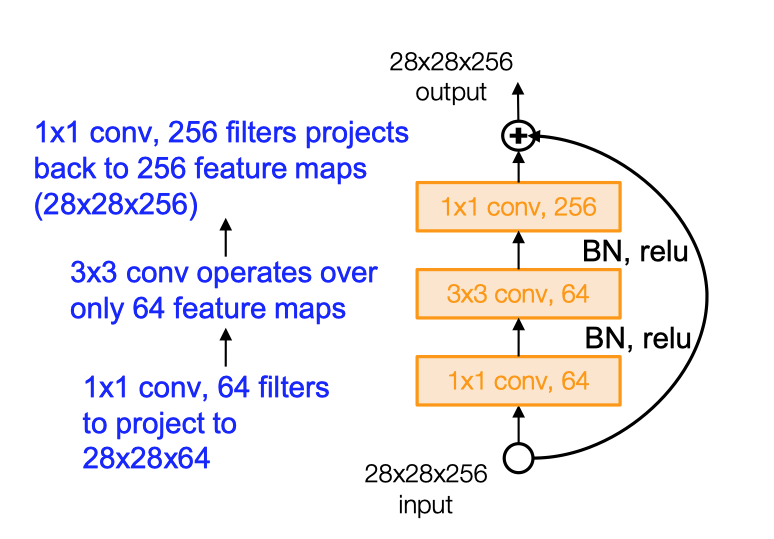
\includegraphics[keepaspectratio, scale=0.27]{pic/res_arch3}
	\end{textblock*}
\end{frame}

\begin{frame}{ResNet At A Glance}
	
	\begin{textblock*}{5cm}(10.5cm,1.3cm) % {block width} (coords)
		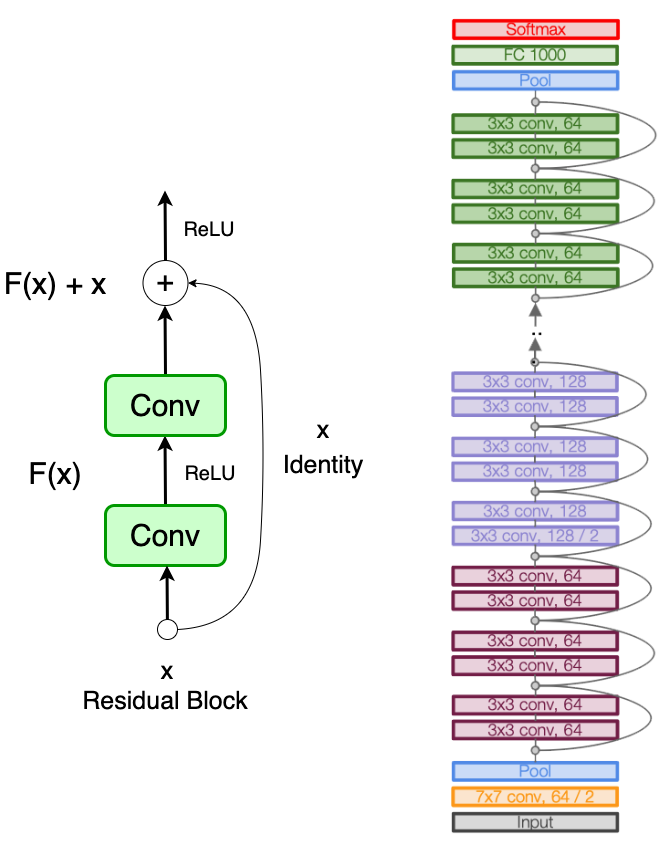
\includegraphics[keepaspectratio, scale=0.23]{pic/resBlock}
	\end{textblock*}
	
	\begin{itemize}
		\item Very deep networks using residual connections
		\item ResNet \textbf{introduces} the concept of skip connections \newline (or residual connections) that allow the gradient to \newline be directly backpropagated to earlier layers.
		\item \textbf{Skip connections helps overcoming gradient vanishing} \newline problem, where the accuracy saturates and then \newline degrades rapidly as the network depth increases.
		\item 152-layer model for ImageNet
		\item ILSVRC’15 classification winner (3.57 \% top 5 error)
		\item Swept all classification and detection competitions \newline in ILSVRC’15 and COCO’15!
	\end{itemize}
\end{frame}

\begin{frame}{ResNet Experiments}
	\begin{itemize}
		\item Able to train very deep networks without degrading (152 layers on ImageNet, 1202 on CIFAR)
		\item Deeper networks now achieve lower training error as expected.
	\end{itemize}
	\begin{figure}[htpb]
		\begin{center}
			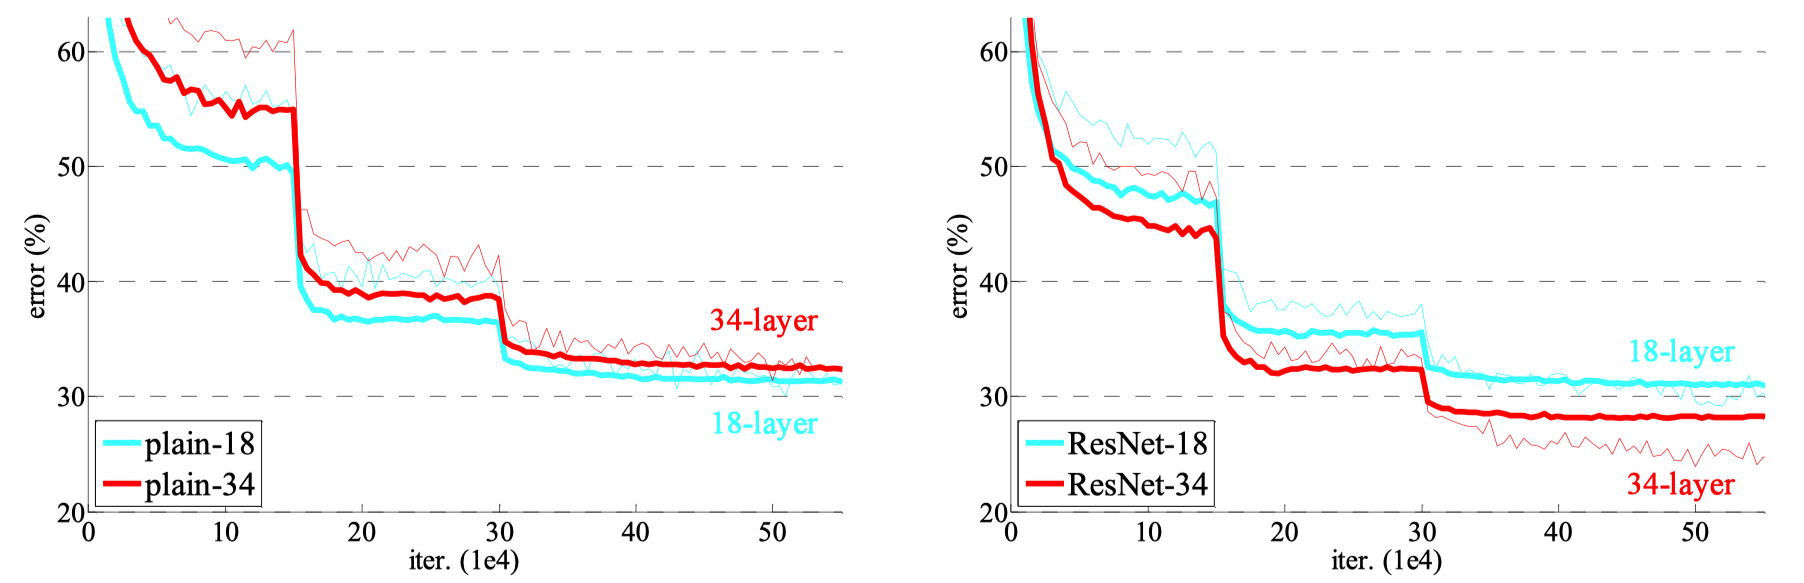
\includegraphics[keepaspectratio, scale=0.2]{pic/ResNetExp}
			\caption*{\scriptsize Thin curves represent training error, and bold curves represent validation error [He, et al. 2015]}
		\end{center}
	\end{figure}
\end{frame}

\begin{frame}{Training ResNet In Practice:}
	\begin{itemize}
		\item Batch Normalization after every CONV layer
		\item Xavier initialization from He, et al.
		\item SGD + Momentum (0.9)
		\item Learning rate: 0.1, divided by 10 when validation error plateaus
		\item Mini-batch size 256
		\item Weight decay of 1e-5
		\item No dropout used
	\end{itemize}
\end{frame}

\begin{frame}{Key Points}
	\begin{itemize}
		\item \textbf{AlexNet} showed that you can use CNNs to train Computer Vision models. 
		\item \textbf{ResNet} showed us how to train extremely deep networks.
		\setbeamertemplate{itemize subitem}{$\rightarrow$}
		\begin{itemize}
			\item Limited only by GPU \& memory!
			\item Showed diminishing returns as networks got bigger (increasing the depth or size of the network doesn't proportionally improve its performance)
		\end{itemize}
		\item After ResNet: CNNs were better than the human metric and focus shifted to other topics:
		\setbeamertemplate{itemize subitem}{$\star$}
		\begin{itemize}
			\item Efficient Networks: \textbf{MobileNet, ShuffleNet}
			\item \textbf{Neural Architecture Search} can now automate architecture design
		\end{itemize}
	\end{itemize}
\end{frame}

\section{Data Preprocessing}

\begin{frame}{Normalizing The Data}
	\begin{itemize}
		\item Assume $X_{n \times d}$ is data matrix, with each sample  is represented in a row
		\item $i$ is the index of dimension (\ $i = 1, \dots d$\ )
	\end{itemize}
	\begin{figure}[htpb]
		\begin{center}
			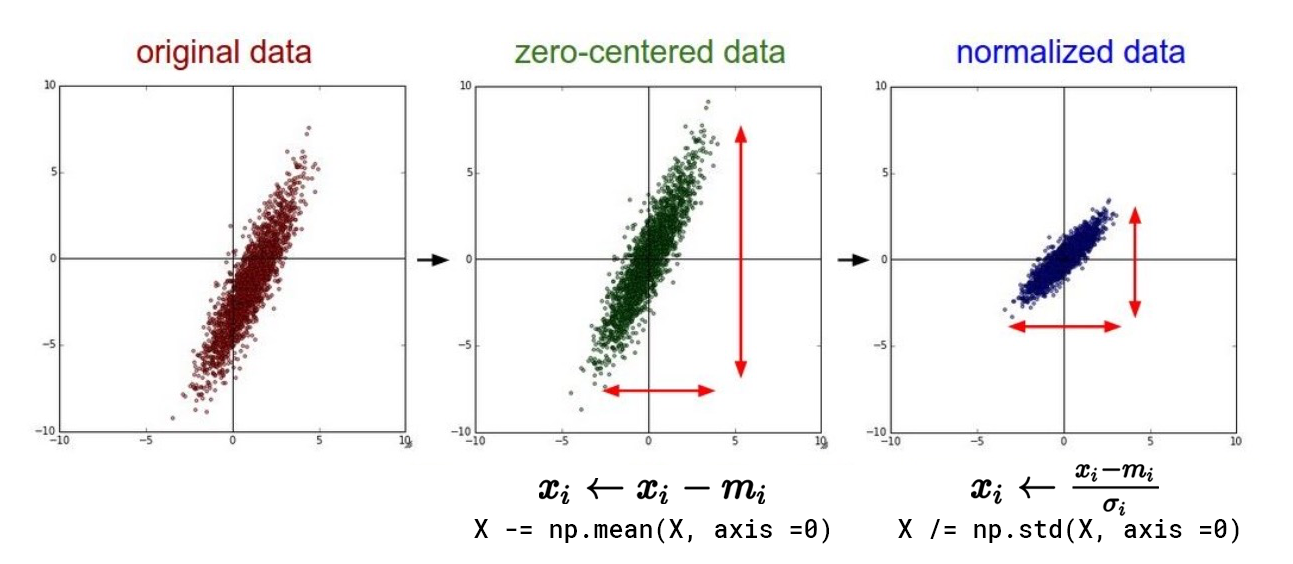
\includegraphics[keepaspectratio, scale=0.3]{pic/normaliz}
		\end{center}
	\end{figure}
\end{frame}

\begin{frame}{TLDR: In Practice For Images: Center Only}
	\begin{itemize}
		\item Example: consider CIFAR-10 example with $[32,32,3]$ images
		\item 3 different approaches:
		\begin{enumerate}
		\item Subtract the mean image (e.g. AlexNet)
			\begin{itemize}
				\item mean image = $[32,32,3]$ array
			\end{itemize}
		\item Subtract per-channel mean (e.g. VGGNet)
			\begin{itemize}
				\item mean along each channel = 3 numbers
			\end{itemize}		
		\item Subtract per-channel mean and divide by per-channel std (e.g. ResNet)
		\end{enumerate}
	\end{itemize}
\end{frame}

\begin{frame}{Why Zero-Mean The Input?}

	\begin{textblock*}{5cm}(10cm,2cm) % {block width} (coords)
		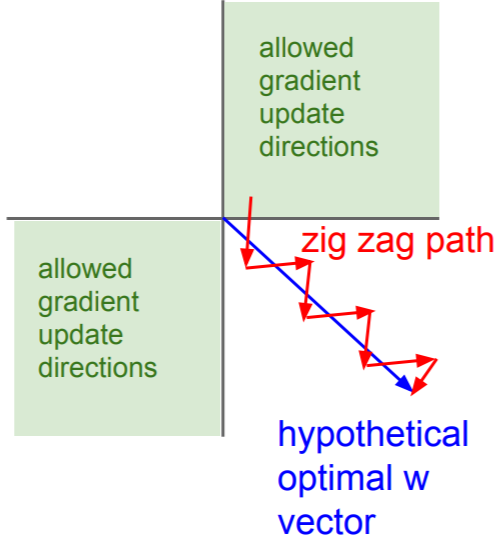
\includegraphics[keepaspectratio, scale=0.3]{pic/zigzag}
	\end{textblock*}

	\begin{itemize}
		\item Reminder: sigmoid
		\item Consider what happens when the input \newline to a neuron is always positive
		\item What can we say about the gradients on w? 
		\begin{itemize}
			\item Always all positive or all negative
			\item Leads to zig-zag dynamics in the gradient updates \newline for the weights (in red) if the optimal $w$ vector was \newline the blue one
		\end{itemize}

		\item This is also why zero-mean data is preferable.
	\end{itemize}
	
\end{frame}

\begin{frame}{Why Normalize The Input?}
	
	\begin{textblock*}{5cm}(9cm,1.5cm) % {block width} (coords)
		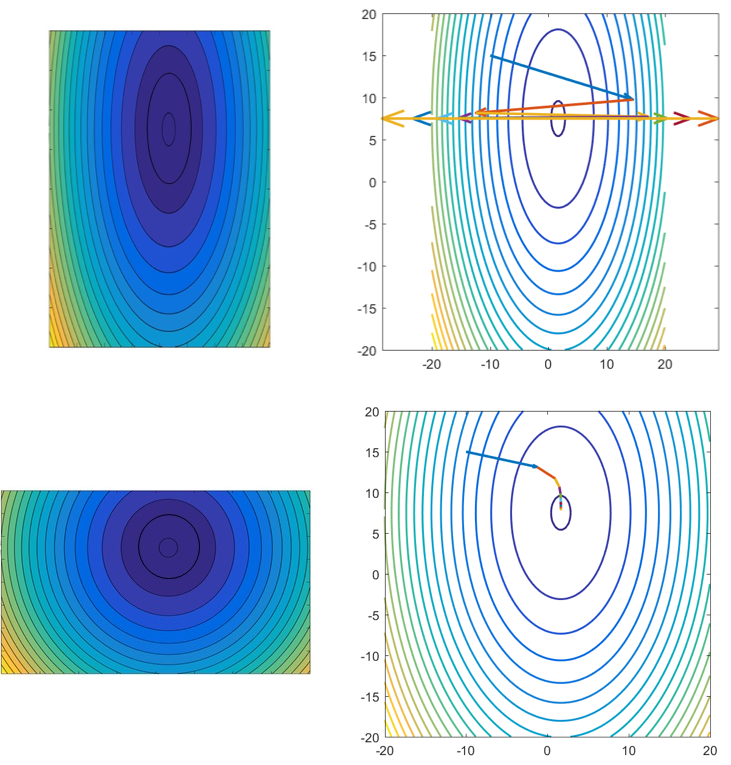
\includegraphics[keepaspectratio, scale=0.25]{pic/poorcond}
	\end{textblock*}
	
	\begin{itemize}
		\item Wide variation in the range of feature \newline values
		\begin{itemize}
			\item Leads to poor conditioning
		\end{itemize}
		\item Results in noisy movement of gradient
	\end{itemize}
	\vspace{1.5cm}
	\begin{itemize}
		\item Normalized data:
		\begin{itemize}
			\item Enhances the geometry of the loss \newline function
			\begin{itemize}
				\item Mitigates issues of poor conditioning
			\end{itemize}
			\item Accelerates convergence during training
		\end{itemize}
	\end{itemize}
\end{frame}


\begin{frame}
	\begin{itemize}
		\item While standardizing inputs is common practice, transformations like variance normalization, PCA, and whitening are used more selectively.
	\end{itemize}
	\begin{figure}[htpb]
		\begin{center}
			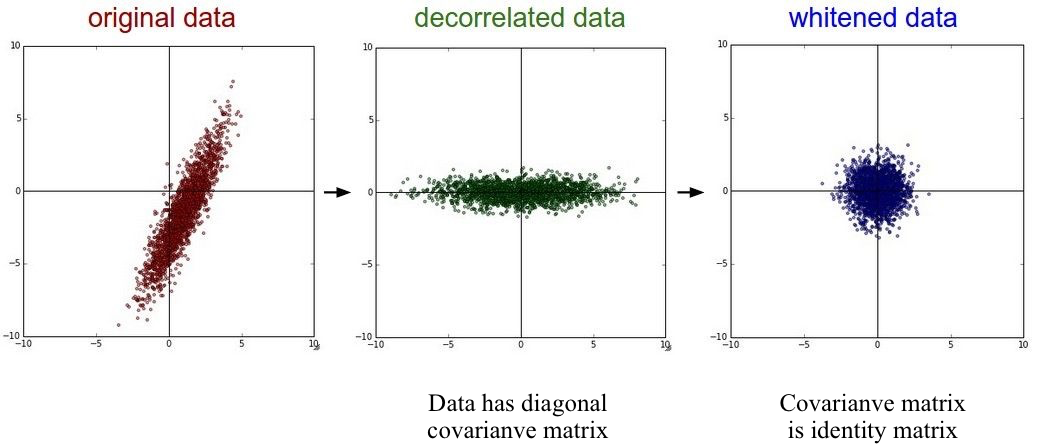
\includegraphics[keepaspectratio, scale=0.35]{pic/whiten}
		\end{center}
	\end{figure}	
\end{frame}

\section{Data Augmentation}

\begin{frame}{Motivation}
	\begin{textblock*}{5cm}(7.2cm,3.7cm) % {block width} (coords)
		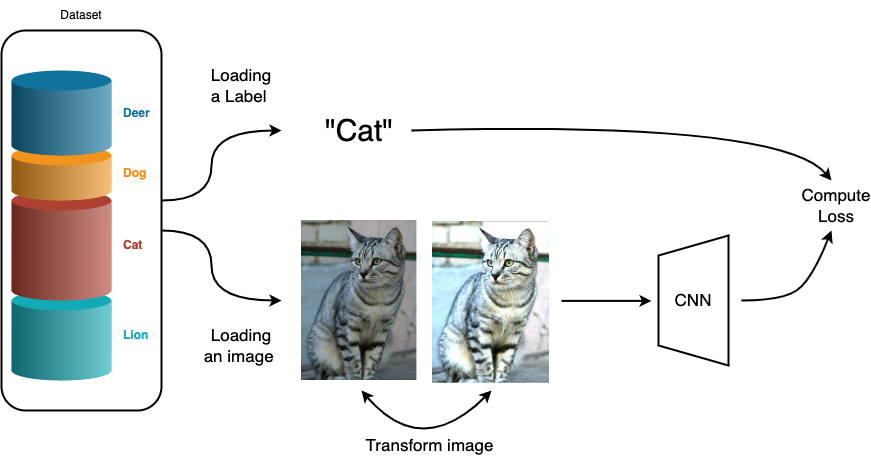
\includegraphics[keepaspectratio, scale=0.28]{pic/cnnaug}
	\end{textblock*}
	
	\begin{itemize}
		\item Getting more training data is often expensive
		\item But, we can often generate additional training examples from existing datasets.
		\item Transform each input data example in such a way that the label stays the same
		\item Benefits:
		\begin{itemize}
			\item Reduces the risk of overfitting
			\item Improves generalization
			\item Acts as a regularization
		\end{itemize}
		\item Examples of data augmentations
		\begin{itemize}
			\item Translation
			\item Flip (Horizontal/Vertical)
			\item Rotation
			\item Stretching
			\item Shearing
			\item Lens distortions, … (going crazy)
		\end{itemize}
	\end{itemize}
\end{frame}

\begin{frame}{Augmentations In Action}
	\begin{textblock*}{6cm}(9cm,2.2cm) % {block width} (coords)
		\begin{figure}
			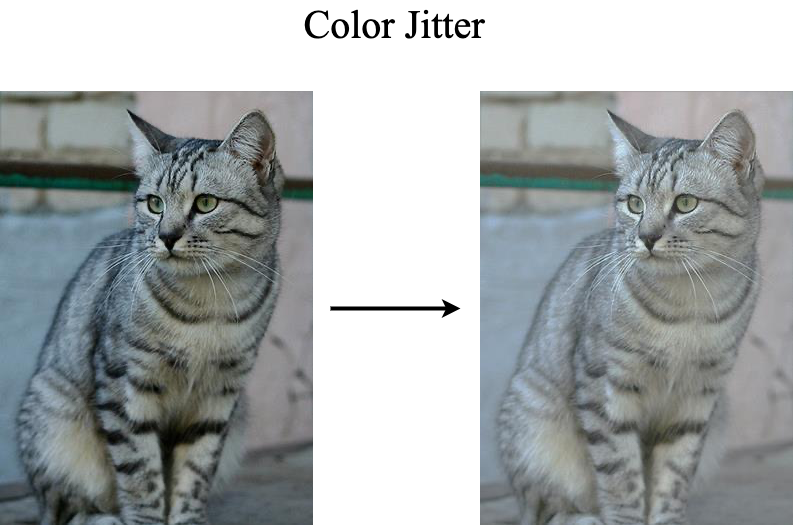
\includegraphics[keepaspectratio, scale=0.22]{pic/jitter}
			\caption*{\tiny{\href{https://www.flickr.com/photos/malfet/1428198050}{\color{blue} This image} by \href{https://www.flickr.com/photos/malfet/}{\color{blue} Nikita} is licensed under \href{https://creativecommons.org/licenses/by/2.0/}{\color{blue} CC-BY 2.0}}}
		\end{figure}

	\end{textblock*}
	
	\begin{itemize}
		\item Simple
		\begin{itemize}
			\item Randomize contrast and brightness levels
		\end{itemize}
		\item Complex
		\begin{enumerate}
			\item Apply PCA to all [R, G, B] pixels \newline in training set
			\item Sample a “color offset” along principal \newline component directions
			\item Add offset to all pixels of a training \newline image
			\newline \small{(As seen in AlexNet, ResNet, etc)}
		\end{enumerate}
	\end{itemize}
\end{frame}

\begin{frame}{Augmentations In Action}
	\begin{textblock*}{5cm}(10cm,2.2cm) % {block width} (coords)
		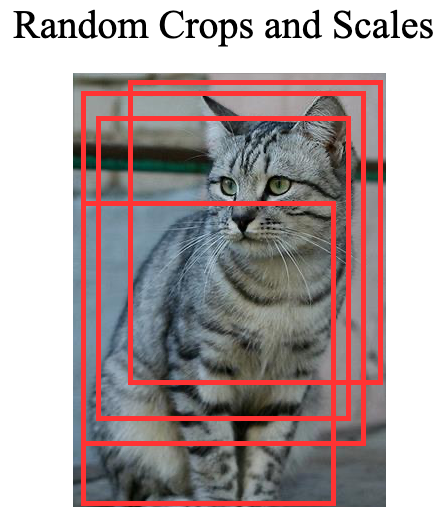
\includegraphics[keepaspectratio, scale=0.28]{pic/crop}
	\end{textblock*}

	\begin{itemize}
	\item \textbf{Training:} randomly sample crops and scales \newline ResNet:
		\begin{enumerate}
				\item Pick random L in range [256, 480]
				\item Resize training image, short side = L
				\item Sample random 224 x 224 patch
		\end{enumerate}
		
	\item \textbf{Testing:} average a fixed set of crops \newline ResNet:
		\begin{enumerate}
			\item Resize image at 5 scales: {224, 256, 384, 480, 640}
			\item For each size, use 10 224 x 224 crops: \newline 4 corners + center + flips
		\end{enumerate}				
	\end{itemize}
\end{frame}


\begin{frame}{Augmentations In Action}
	\begin{textblock*}{5cm}(10cm,1.5cm) % {block width} (coords)
		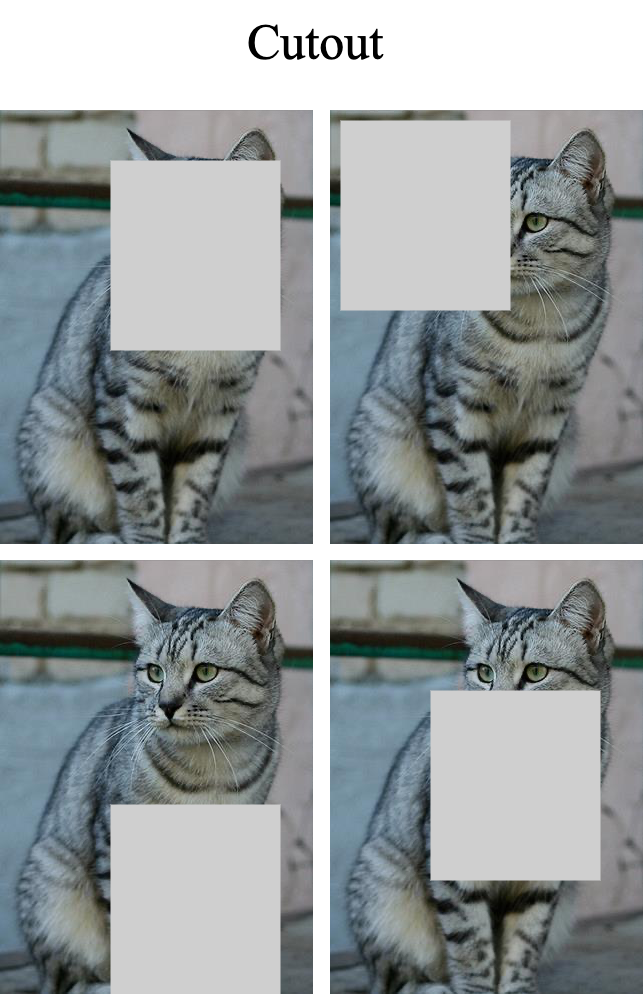
\includegraphics[keepaspectratio, scale=0.18]{pic/cutout.png}
	\end{textblock*}

	\begin{itemize}
		\item \textbf{Training:} Randomly set image regions to zero
		\item \textbf{Testing:} Use the full image
		\item Effective for  small datasets like CIFAR, less \newline common for large datasets like ImageNet
	\end{itemize}

	\begin{textblock*}{10cm}(1.5cm,8.2cm) % {block width} (coords)
		\tiny{DeVries and Taylor, ``Improved Regularization of Convolutional
		Neural Networks with Cutout'', arXiv 2017}
	\end{textblock*}
\end{frame}

\begin{frame}[fragile]{Augmentation With Albumentations}

\begin{minipage}{0.43\textwidth}
\begin{lstlisting}[language=python]
import albumentations as A
\end{lstlisting}
\end{minipage}

	
	\begin{textblock*}{5cm}(10cm,1.7cm) % {block width} (coords)
		
\includegraphics[keepaspectratio, width=5cm]{pic/Albumentations}
	\end{textblock*}
	
	\vspace{0.5cm}
	\begin{itemize}
		\item Basic pixel-Level Augmentations
		\begin{itemize}
			\item 
			{\sffamily A.RandomBrightnessContrast(),A.HueSaturationValue(), 
				A.GaussianBlur()}
		\end{itemize}
		
		\item Image Distortion and Warping
		\begin{itemize}
			\item {\sffamily A.ElasticTransform(), A.GridDistortion(), A.OpticalDistortion()}
		\end{itemize}
		\item And many more:
		\begin{itemize}
			\item Advanced Pixel-Level Augmentations, Cropping and Padding, Geometric Transformations, Composite Augmentations, etc.
		\end{itemize}
		\item Albumentations can even be used to \textbf{augment bounding boxes for object detection tasks} (check \href{https://albumentations.ai/docs/examples/example_bboxes/}{\color{blue}this} out!)
		\item Interactive demo: \href{https://demo.albumentations.ai}{\color{blue} https://demo.albumentations.ai}

	\end{itemize}
\end{frame}

\begin{frame}{Examples}	

	\begin{figure}
		\begin{center}
			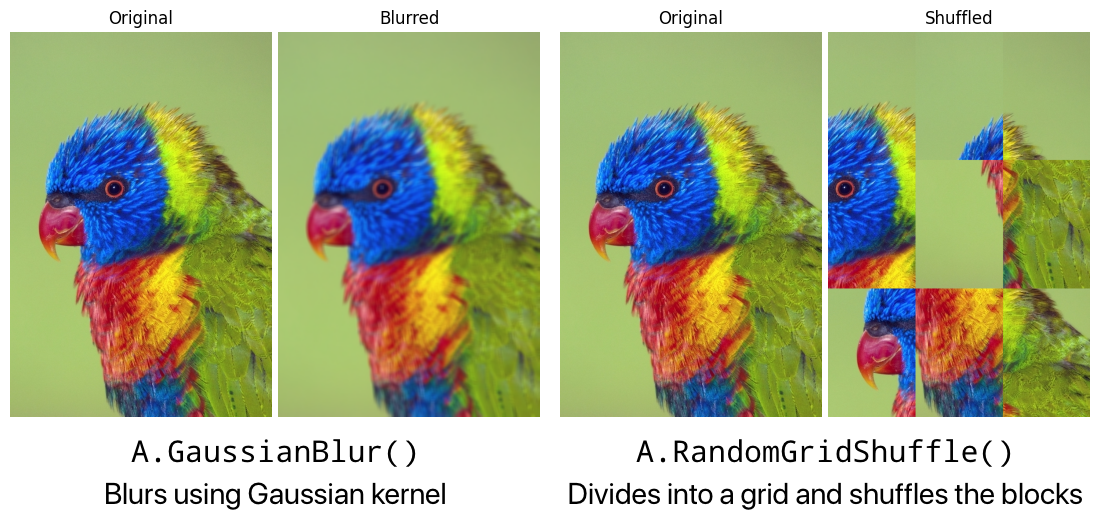
\includegraphics[keepaspectratio, scale=0.3]{pic/Albu_example}
			\caption*{Image source: \href{http://freepik.com}{\color{blue}freepik.com}}
		\end{center}
	\end{figure}
\end{frame}

\section{Transfer Learning}
\begin{frame}{Motivation}
	\begin{itemize}
		\item You need a lot of a data if you want to train/use CNNs
		\item Suppose you want to build an app to recognize flowers…
	\end{itemize}
	\begin{figure}[htpb]
		\begin{center}
			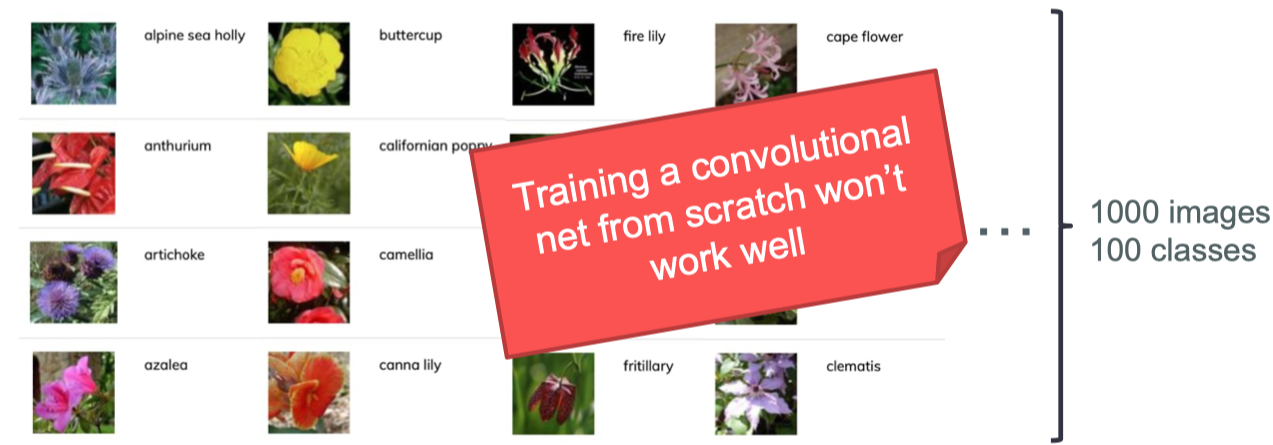
\includegraphics[keepaspectratio, scale=0.25]{pic/TL_motiv}
			\caption*{\scriptsize https://www.robots.ox.ac.uk/~vgg/data/flowers/102}
		\end{center}
	\end{figure}
\end{frame}

\begin{frame}{Transfer Learning}
	\begin{enumerate}
		\item Pretrain on a large dataset (e.g. ImageNet)
		\item Fine-tune it on a small target dataset (e.g. Flowers)
	\end{enumerate}

	\begin{figure}
		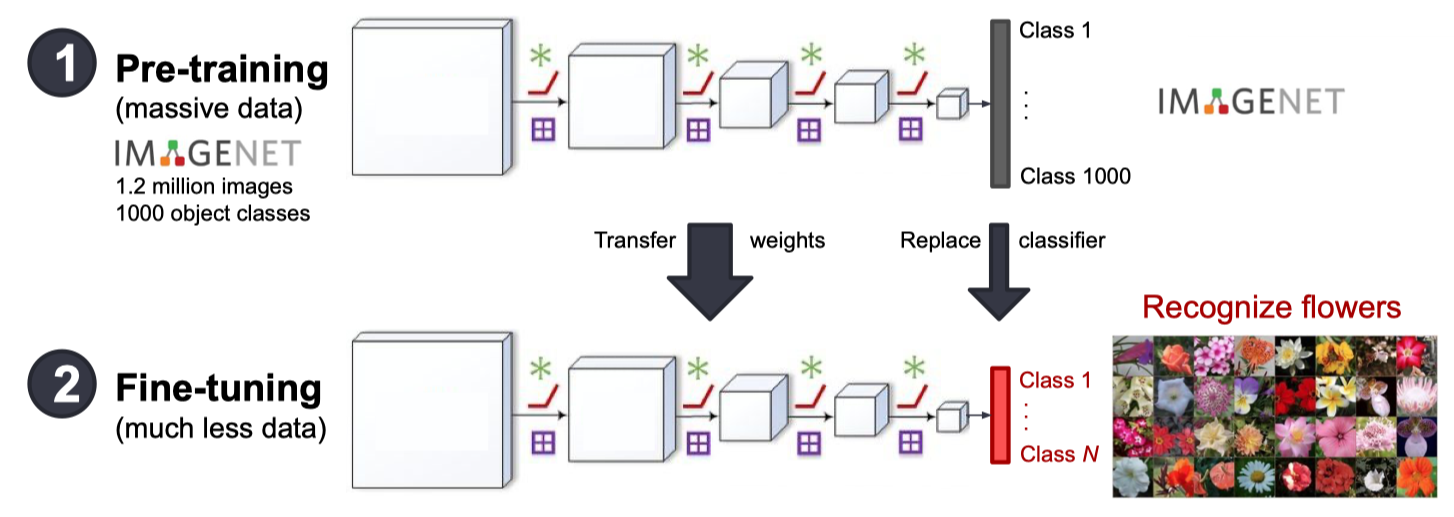
\includegraphics[keepaspectratio, scale=0.23]{pic/TL_idea}
	\end{figure}
\end{frame}

\begin{frame}{Transfer Learning: The idea}
	\vspace{-1em}
	\begin{figure}[htpb]
		\begin{center}
			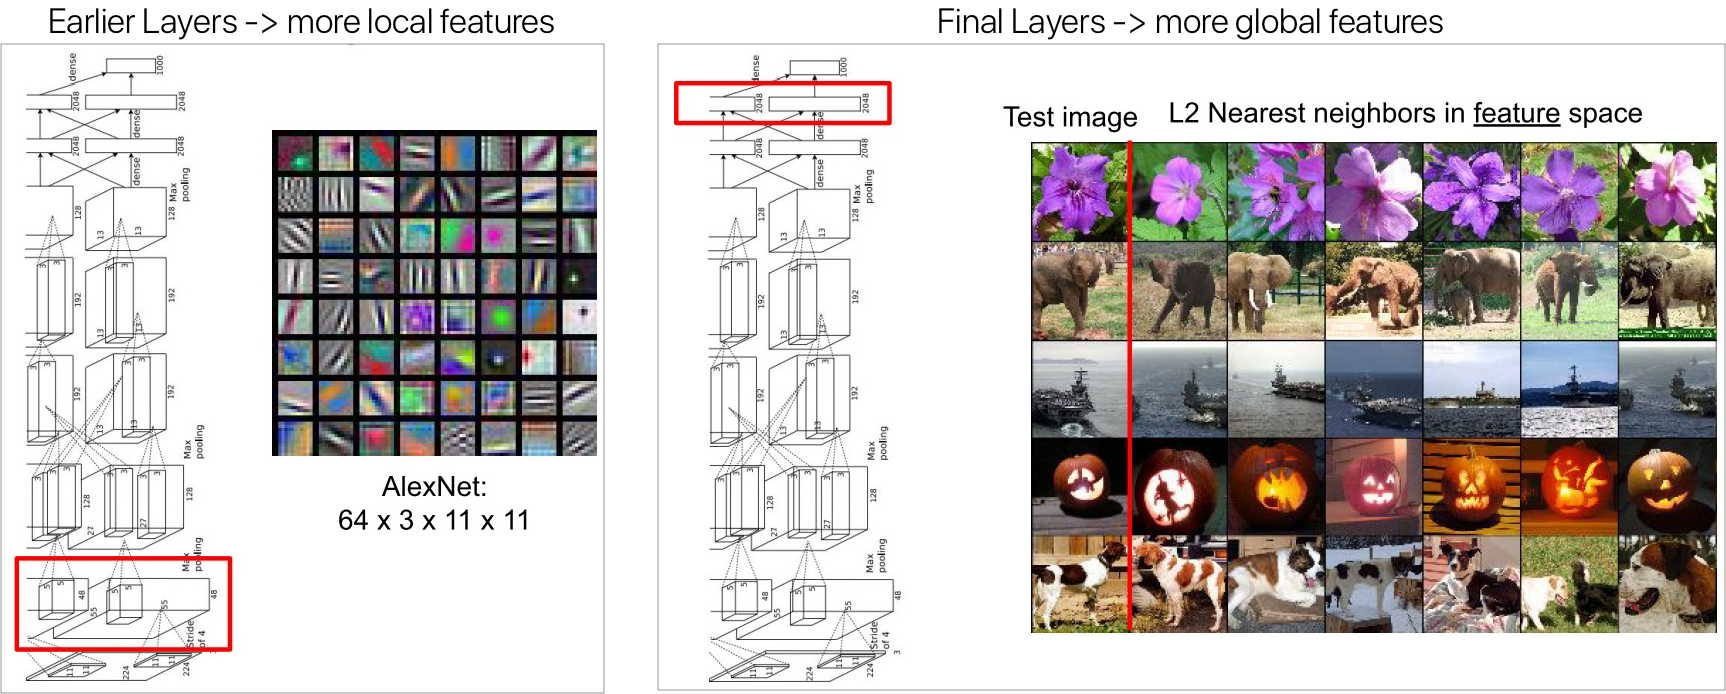
\includegraphics[keepaspectratio, scale=0.23]{pic/TL_alexnet}
		\end{center}
	\end{figure}
\end{frame}

\begin{frame}{Transfer Learning With CNNs}
	\begin{figure}[htpb]
		\begin{center}
			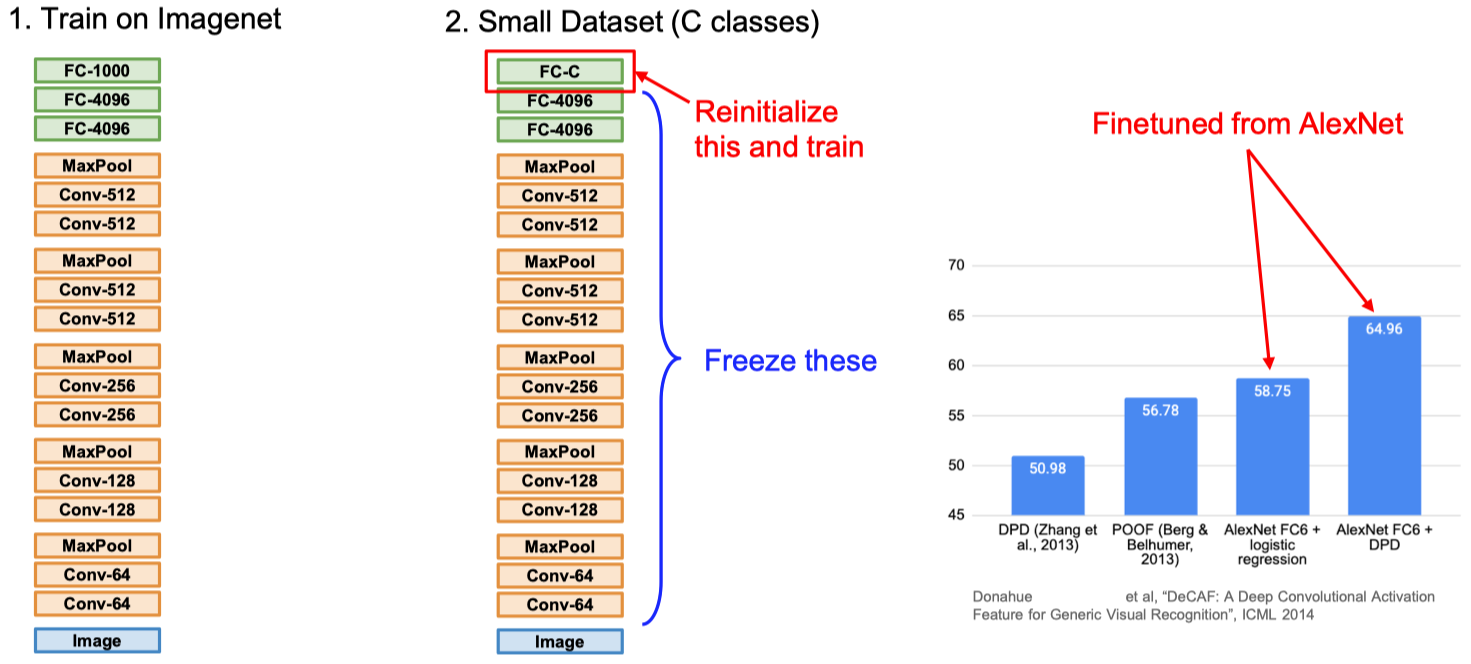
\includegraphics[keepaspectratio, scale=0.25]{pic/TL_cnn}
			\caption*{\scriptsize Donahue et al, (ICML 2014), Razavian et al, (CVPR Workshops 2014)}
		\end{center}
	\end{figure}
\end{frame}

\begin{frame}{Transfer Learning With CNNs}
	\begin{figure}[htpb]
		\begin{center}
			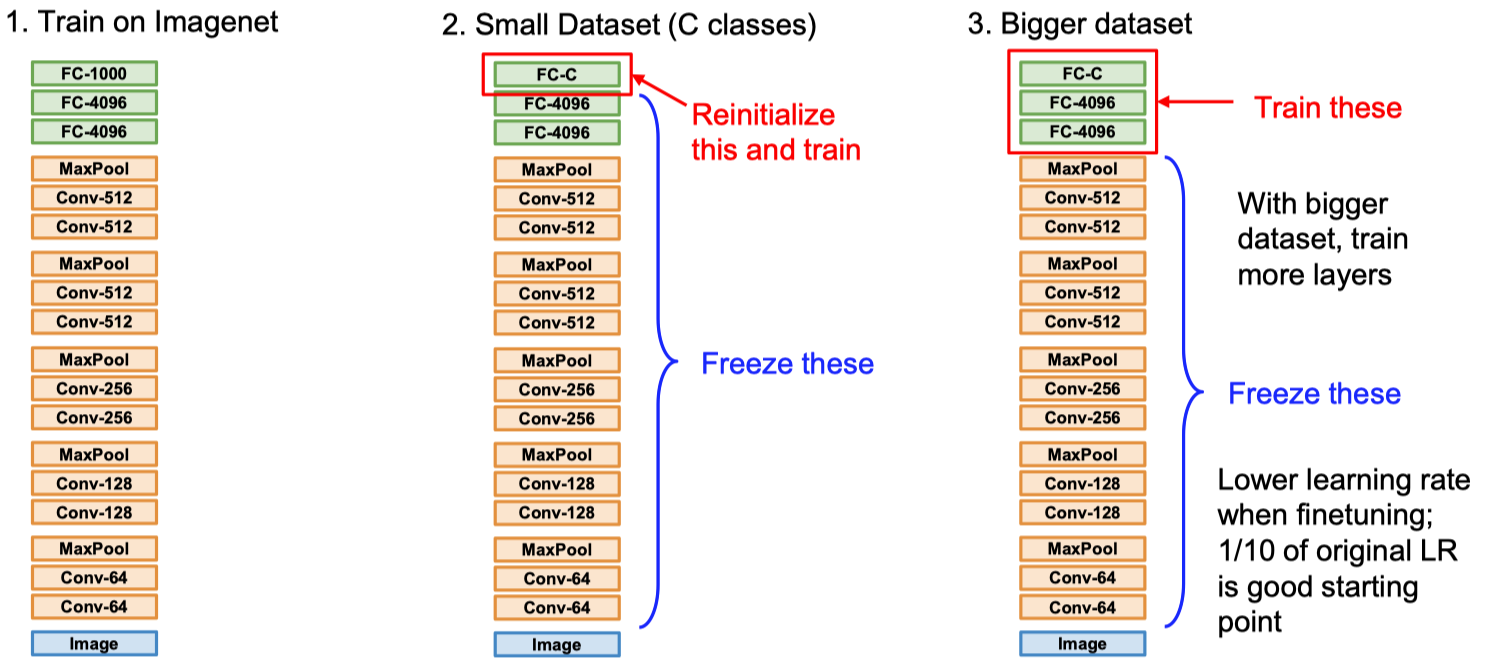
\includegraphics[keepaspectratio, scale=0.25]{pic/TL_cnn2}
		\end{center}
	\end{figure}
\end{frame}

\begin{frame}{Transfer Learning With CNNs}
	\begin{figure}[htpb]
		\begin{center}
			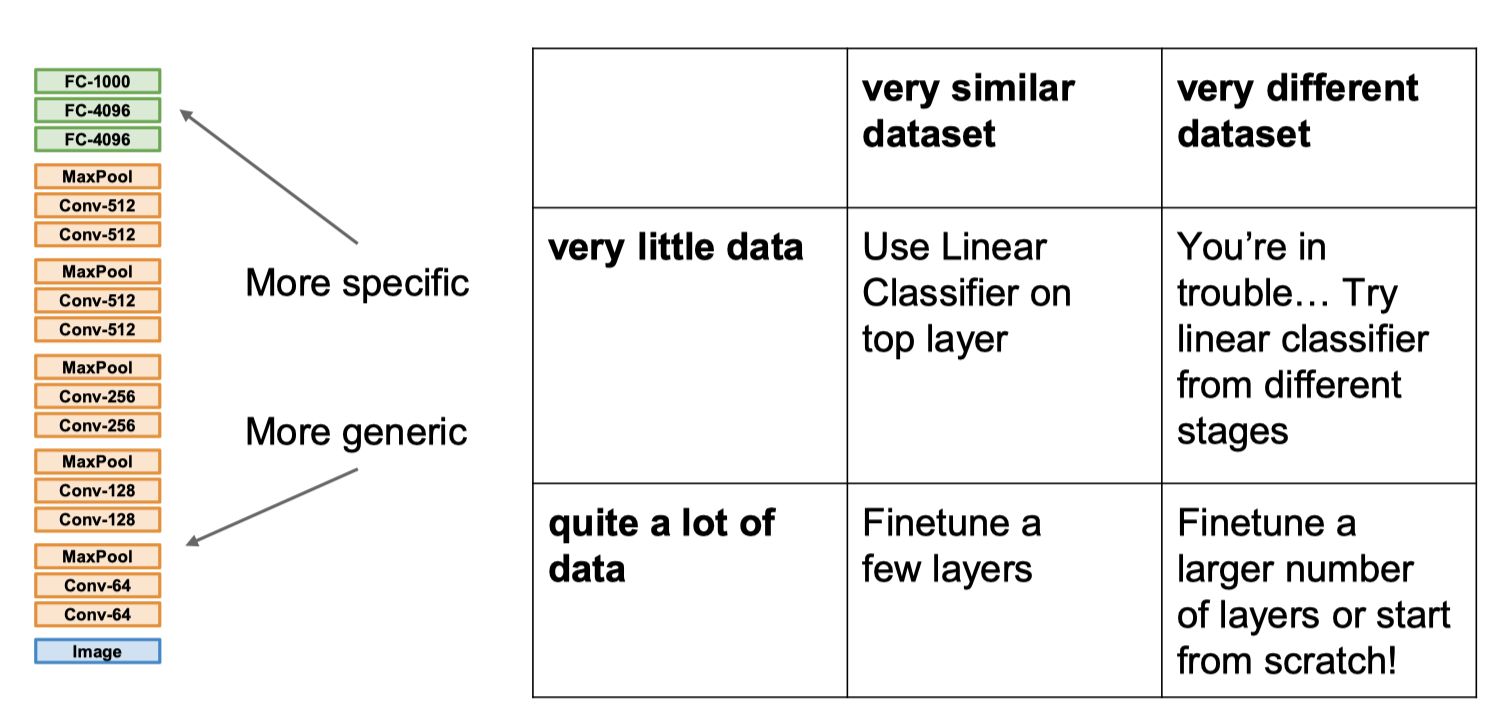
\includegraphics[keepaspectratio, scale=0.25]{pic/TL_cnn3}
		\end{center}
	\end{figure}
\end{frame}

\begin{frame}{Transfer Learning: Domain Shift}
	\begin{figure}[htpb]
		\begin{center}
			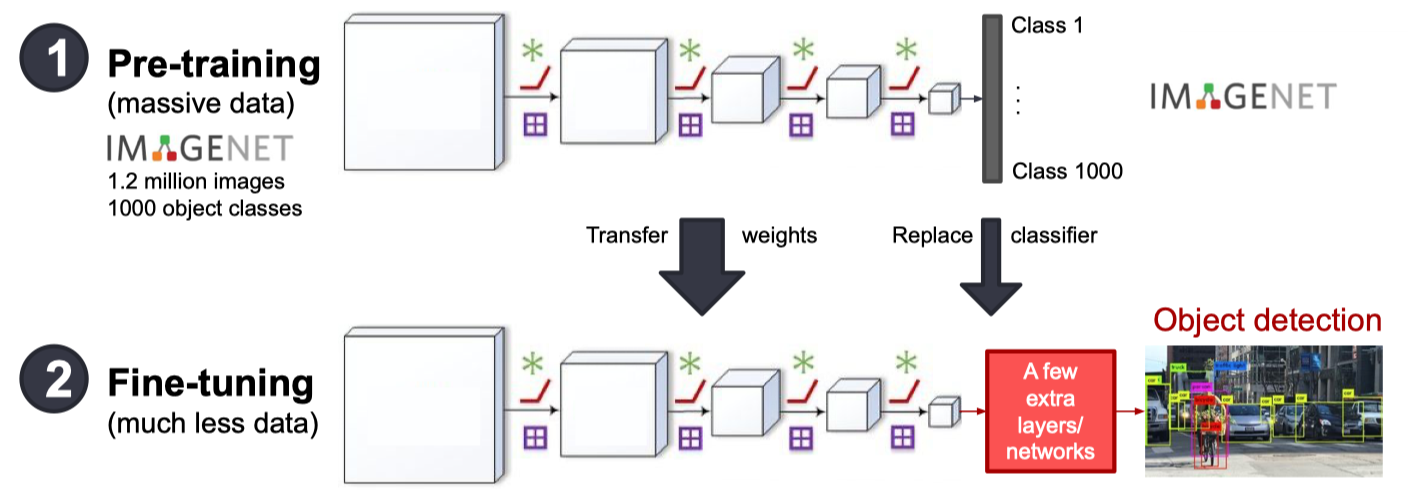
\includegraphics[keepaspectratio, scale=0.25]{pic/TL_domain_change}
		\end{center}
	\end{figure}
\end{frame}

\begin{frame}{Example: Semantic Segmentation}
	\begin{figure}[htpb]
		\begin{center}
			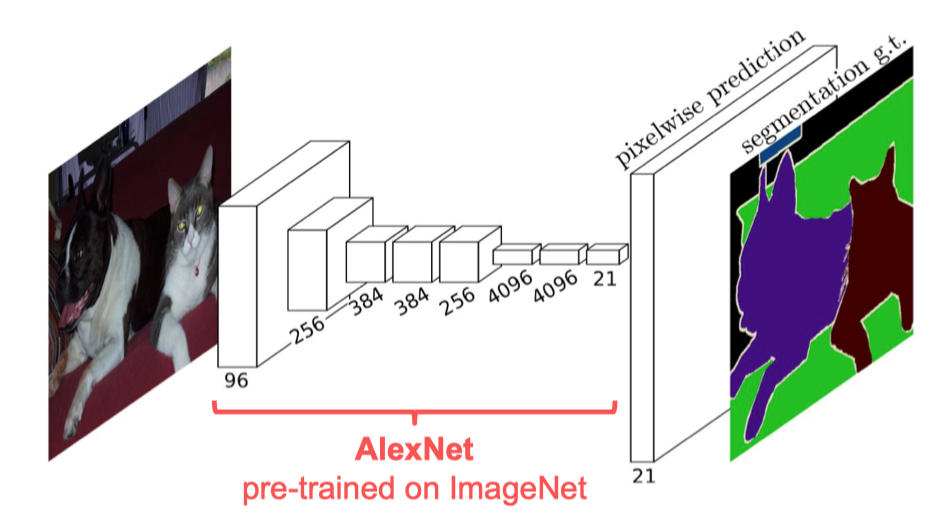
\includegraphics[keepaspectratio, scale=0.25]{pic/sem}
			\caption*{\scriptsize Long, Shelhamer, Darrell, CVPR 2015}
		\end{center}
	\end{figure}
\end{frame}

\begin{frame}{Transfer Learning With CNNs Is Pervasive…}
	\begin{textblock*}{5cm}(0.5cm,1.9cm) % {block width} (coords)
		\begin{center}
			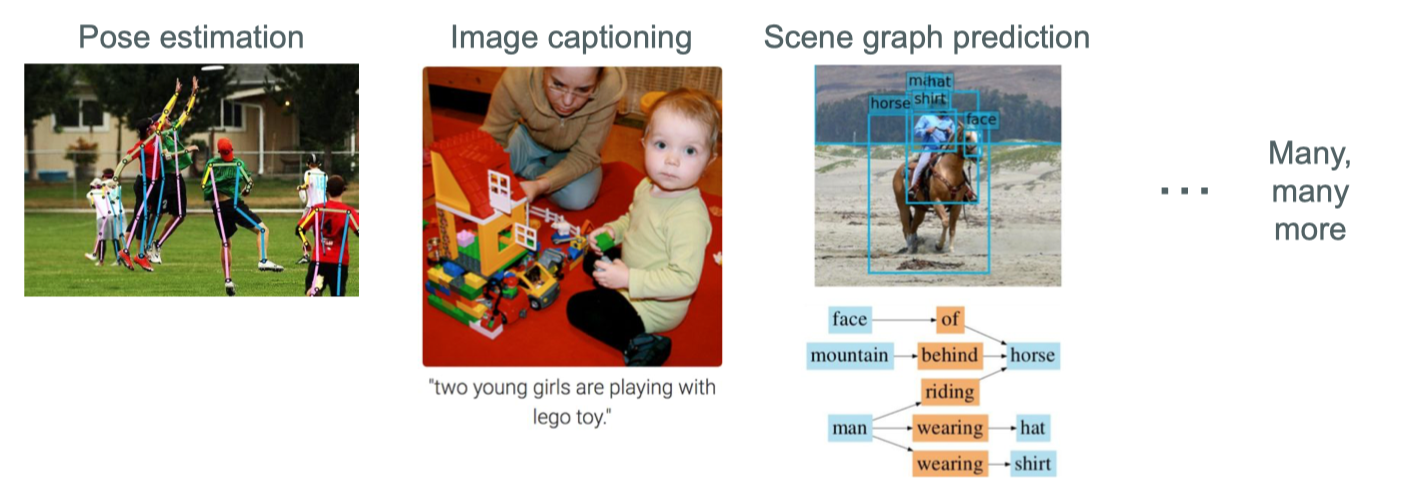
\includegraphics[keepaspectratio, scale=0.31]{pic/TL_examples}
		\end{center}
	\end{textblock*}
\end{frame}

\begin{frame}{Transfer Learning With CNNs Is Pervasive…}
	\begin{figure}[htpb]
		\begin{textblock*}{2cm}(0.5cm,1.7cm) % {block width} (coords)
			\begin{center}
				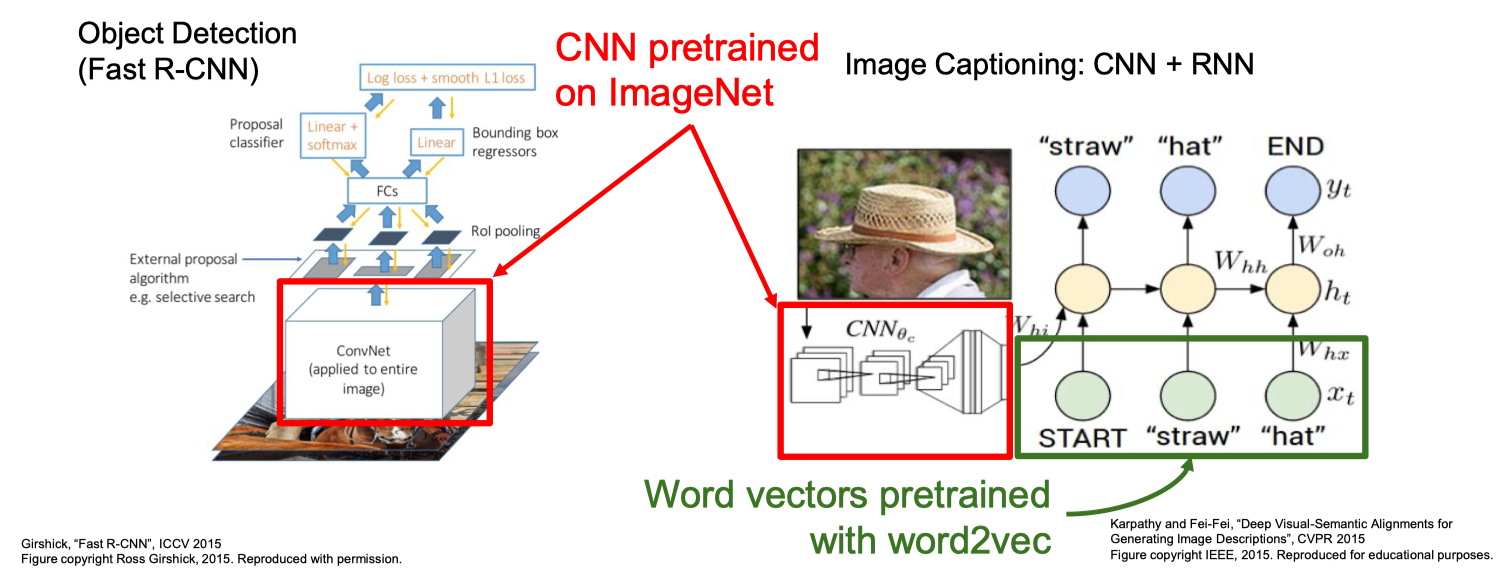
\includegraphics[keepaspectratio, scale=0.29]{pic/TL_examples2}
			\end{center}
		\end{textblock*}
	\end{figure}
\end{frame}

\begin{frame}{Transfer Learning Might Not Always Be Necessary!}
	\begin{itemize}
		\item Training from scratch can perform as well \newline as using a pretrained ImageNet model for \newline object detection.
		\item But it requires 2-3 times longer to train.
		\item Collecting more data is better than \newline finetuning on a related task
	\end{itemize}
	\begin{textblock*}{5cm}(9cm,1.3cm) % {block width} (coords)
		\begin{figure}
			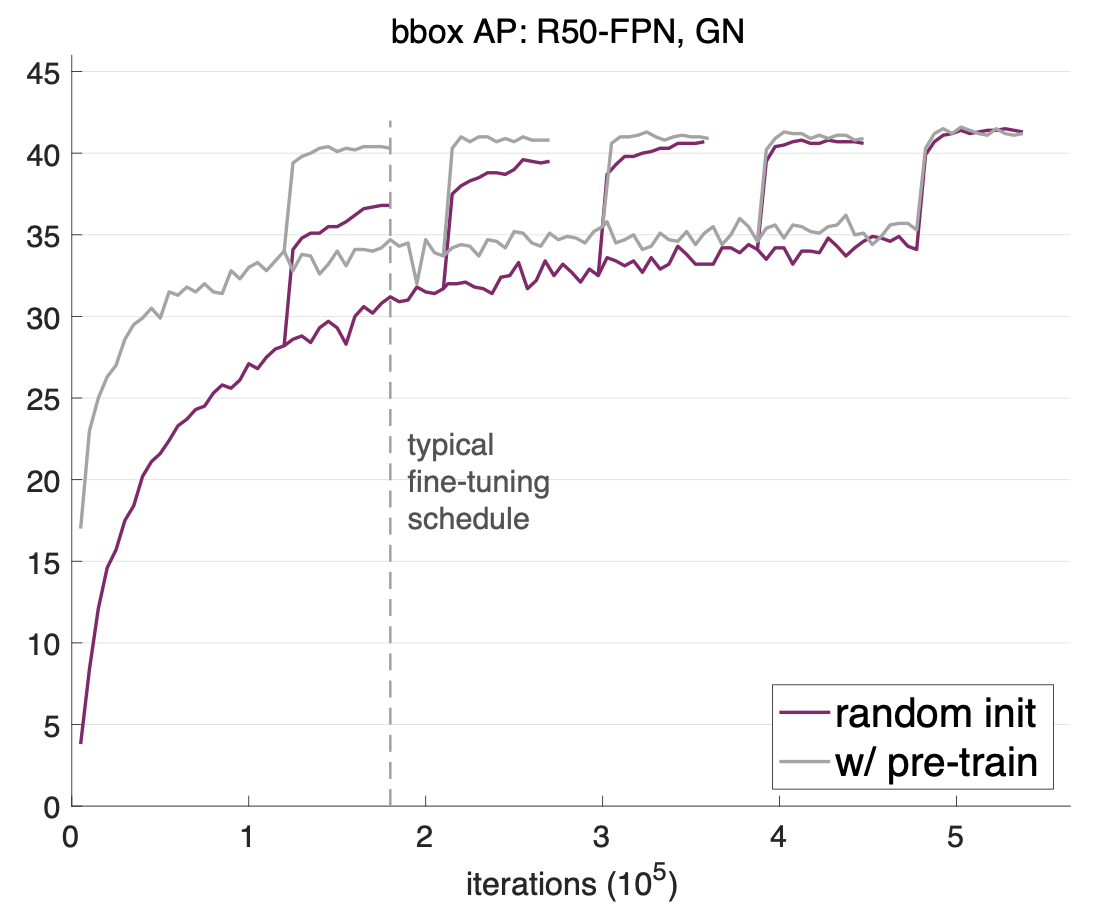
\includegraphics[keepaspectratio, scale=0.35]{pic/rethinking_imagenet}
			\caption*{\hspace{2cm}\scriptsize He et al (ICCV 2019)}
		\end{figure}
	\end{textblock*}
\end{frame}

\begin{frame}{Takehome Message}
	\begin{itemize}
		\item Have some dataset of interest but it has fewer than $\texttildelow$ 1M images?
		\begin{enumerate}
			\item Find a very large dataset that has similar data, train a big ConvNet there
			\item Transfer learn to your dataset
		\end{enumerate}
		\item Deep learning frameworks offer a "Model Zoo" of pretrained models so you don't need to train your own
		\begin{itemize}
			\item \textbf{Pytorch:} \href{https://github.com/pytorch/vision}{\color{blue} https://github.com/pytorch/vision}
			\item \textbf{TensorFlow:} \href{https://github.com/tensorflow/models}{\color{blue} https://github.com/tensorflow/models}
		\end{itemize}

	\end{itemize}
\end{frame}

\section{References}

\begin{frame}
	\textbf{Slides by: Ali Bavafa}
\end{frame}

\begin{frame}
	\nocite{*}
	\bibliographystyle{ieeetr}
	\bibliography{ref}
\end{frame}


\begin{frame}
	\begin{center}
		{\Huge Any Questions?}
	\end{center}
\end{frame}

\end{document}